\chapter{Process Initialization, Creation, and Management}
\mpitermtitleindex{process creation}
\label{sec:dynamic-2}
\label{chap:dynamic-2}

\section{Introduction}
\label{sec:dynamic:introduction}

\mpi/ is primarily concerned with communication rather than process or
resource management.  However, it is necessary to address these issues
to some degree in order to define a useful framework for communication.
This chapter presents a set of \mpi/ interfaces that allows for
several approaches to \MPI/ initialization and
process management while placing minimal
restrictions on the execution environment.

One goal of \MPI/ is to achieve \emph{source code portability}.  By this we mean
that a program written using \MPI/ and complying with the relevant language
standards is portable as written, and must not require any source code changes
when moved from one system to another.  This explicitly does \emph{not} say
anything about how an \MPI/ program is started or launched from the command
line, nor what the user must do to set up the environment in which an \MPI/
program will run.  However, an implementation may require some setup or initialization
procedure to be performed before the complete set of \MPI/ routines may be called.

To this end, \mpi/ presents two models for \mpitermdefni{MPI process initialization}\mpitermdefindex{MPI process initialization@\MPI/ process initialization}.
In the \wpm{}\mpitermindex{MPI process initialization@\MPI/ process initialization!\wpm}\mpitermindex{\wpm},
an initial set of processes is created that are related by their membership in a common
\mpiconst{MPI\_COMM\_WORLD}
(see Section~\ref{sec:dynamic:initialization}) communicator.
In the \spm{}\mpitermindex{MPI process initialization@\MPI/ process initialization!\spm}\mpitermindex{\spm} (Section~\ref{sec:model_sessions}),
an initial set of processes is also created, but the application must explicitly manage the
creation of \MPI/ groups, and hence \MPI/ communicators.
\mpiconst{MPI\_COMM\_WORLD} is only valid for use as a communicator in the \wpm{}, i.e., after a successful
call to \mpifunc{MPI\_INIT} or \mpifunc{MPI\_INIT\_THREAD} and before a call to \mpifunc{MPI\_FINALIZE}.
An application can employ both of these Process Models concurrently.
In multi-component \mpi/ applications, for example, a component such as a library
can make use of the \spm{} to instantiate \MPI/ resources without impacting the rest of the application.

The Dynamic Process Model (see Section~\ref{sec:model}),
provides for
the creation and management of additional processes
after an \mpi/ application has been started.
A major impetus for
the Dynamic Process Model\mpitermindex{MPI process initialization@\MPI/ process initialization!Dynamic Process Model}\mpitermindex{Dynamic Process Model}
comes
from the PVM~\cite{pvmbook} research effort.  This work
has provided a wealth of experience with process
management and resource control that illustrates their benefits
and potential pitfalls.

In developing the Dynamic Process Model, the
\mpi/ Forum decided not to address resource
control because
it was not able to design a portable interface that would be
appropriate for the broad spectrum of existing and potential resource and
process controllers.
\mpi/
assumes that resource control is provided externally.

Process management functionality is included in \MPI/ to enable its use
in classes of message-passing
applications requiring process control. These include task
farms, serial applications with parallel modules, and problems that
require a run-time assessment of the number and type of processes that
should be started.

The following goals are central to the design of \mpi/ process management:

\begin{itemize}

\item The
\mpi/
process model must apply
to the vast majority of current parallel environments.

\item \MPI/ must not take over operating system responsibilities.
It should instead provide a clean interface between an application
and system software.

\item \MPI/ must guarantee communication determinism in the presence of
dynamic processes, i.e.,
dynamic process management must not introduce unavoidable race
conditions.

\item \MPI/ must not contain features that compromise performance.

\end{itemize}

The
Dynamic Process Model
addresses these issues in two
ways. First, \MPI/ remains primarily a communication library. It
does not manage the parallel environment in which
a parallel program executes, though it provides a minimal
interface between an application and external resource and
process managers.

Second, \mpi/ maintains a consistent concept of a communicator, regardless
of how its members came into existence.
A communicator is never changed once created, and it is always
created using deterministic collective operations.

\section{The \texorpdfstring{\wpm}{World Model}}
\label{sec:dynamic:initialization}

%%%%%%%%%%%%%%%%%%%%%%%%%%%%%%%%%%%%%%%%%%%%%%%%%%%%%%%%%%%%%%%%%%%%%%
\subsection{Starting \texorpdfstring{\mpi/}{MPI} Processes}
\mpitermtitleindex{startup}
\label{sec:inquiry-startup}

\label{sec:misc-init}

When using the \wpm{}, \MPI/ is initialized by calling
either \mpifunc{MPI\_INIT} or \mpifunc{MPI\_INIT\_THREAD}.

\begin{mpi-binding}
    function_name("MPI_Init")

    parameter(
        "argc",
        "ARGUMENT_COUNT",
        direction="inout",
        suppress="lis_parameter f08_parameter f90_parameter",
    )
    parameter(
        "argv",
        "ARGUMENT_LIST",
        length="argc",
        pointer=True,
        direction="inout",
        suppress="lis_parameter f08_parameter f90_parameter",
    )
\end{mpi-binding}

In the \wpm{},  an \MPI/ program must contain exactly one call to an \MPI/ initialization routine:
\mpifunc{MPI\_INIT} or \mpifunc{MPI\_INIT\_THREAD}. \mpiconst{MPI\_COMM\_WORLD} and \mpiconst{MPI\_COMM\_SELF} are not valid for use as communicators
prior to invocation of \mpifunc{MPI\_INIT} or \mpifunc{MPI\_INIT\_THREAD}.  Subsequent calls to either of these
initialization routines are erroneous. A subset of \MPI/ functions may be invoked
before \MPI/ initialization routines are called, see \sectionref{subsec:dynamic:preinit_functions}.
The procedures \cfunc{MPI\_INIT} and \cfunc{MPI\_INIT\_THREAD} accept either the \mpiarg{argc} and \mpiarg{argv} that are provided by the arguments to
\code{main} or \code{NULL}.
\begin{example}
\Exindex[Initializing \MPI/]{C}{Initializing MPI@Initializing \MPI/}{MPI\_Init}%
Initializing \MPI/ using \mpifunc{MPI\_INIT}
%%HEADER
%%LANG: C
%%ENDHEADER
\begin{lstlisting}[language={[MPI]C}]
int main(int argc, char *argv[])
{
    MPI_Init(&argc, &argv);

    /* parse arguments */
    /* main program    */

    MPI_Finalize();     /* see below */
    return 0;
}
\end{lstlisting}
\end{example}
The Fortran version takes only \farg{IERROR}.

Conforming implementations of \MPI/ are required to allow
applications to pass \code{NULL} for both the \mpiarg{argc} and
\mpiarg{argv} arguments of \cfunc{main} in
C.

\mpitermindex{error handling!startup}
Failures may disrupt the execution of the program before
or during \MPI/ initialization. A high-quality implementation shall
not deadlock during \MPI/ initialization, even in the presence of failures.
Except for functions with the \mpicode{MPI\_T\_} prefix, failures in \MPI/ operations prior to or during \MPI/ initialization are reported by invoking
the initial error handler.\mpitermindex{error handling!initial error handler} Users can use the \infokey{mpi\_initial\_errhandler} info key
during the launch of \MPI/ processes (e.g., \mpifunc{MPI\_COMM\_SPAWN}, \mpifunc{MPI\_COMM\_SPAWN\_MULTIPLE}, or \mpilaunch{mpiexec}) to set a nonfatal initial error handler before \MPI/ initialization.
When the initial error handler is set to \mpiconst{MPI\_ERRORS\_ABORT},
raising an error before or during initialization aborts the local
\MPI/ process (i.e., it is similar to calling \mpifunc{MPI\_ABORT}
on \mpiconst{MPI\_COMM\_SELF}).
%
An implementation may not always be capable of determining,
before \MPI/ initialization, what constitutes the local \MPI/ process, or the set of
connected processes. In this case, errors before initialization may cause a different set
of \MPI/ processes to abort than specified.
%
During \MPI/ initialization, the initial error handler is associated with
\mpiconst{MPI\_COMM\_WORLD}, \mpiconst{MPI\_COMM\_SELF},
and the communicator returned by \mpifunc{MPI\_COMM\_GET\_PARENT} (if any).

\begin{implementors}
Some failures may leave \MPI/ in an undefined state, or raise an error
before the error handling capabilities are fully operational, in which cases
the implementation may be incapable of providing the desired error handling
behavior. Of note, in some implementations, the notion of an \MPI/ process
is not clearly established in the early stages of \MPI/ initialization (for
example, when the implementation considers threads that called \mpifunc{MPI\_INIT}
as independent \MPI/ processes); in this case, before \MPI/ is initialized,
the \mpiconst{MPI\_ERRORS\_ABORT} error handler may abort what would have become
multiple \MPI/ processes.

When a failure occurs during \MPI/ initialization,
the implementation may decide to return \error{MPI\_SUCCESS} from the \MPI/ initialization function
instead of raising an error.
It is recommended that an implementation
masks an initialization error only when it
expects that later \MPI/ calls will result in well-specified behavior (i.e., barring
additional failures, either the outcome of any call will be correct, or the call
will raise an appropriate error).
For example, it may be difficult for an implementation to
avoid unspecified behavior
 when the group of \mpiconst{MPI\_COMM\_WORLD} does not contain
the same set of \MPI/ processes at all members of the communicator, or if the communicator
returned from \mpifunc{MPI\_COMM\_GET\_PARENT} was not initialized correctly.
\end{implementors}

After \MPI/ is initialized, the application can access information
about the execution environment by querying the predefined info object
\mpiconstmain{MPI\_INFO\_ENV}.
The following keys are predefined for this object, corresponding to the
arguments of \mpifunc{MPI\_COMM\_SPAWN} or of \mpilaunch{mpiexec}:
\begin{description}
\item[\infokeymain{command}:] Name of program executed.
\item[\infokeymain{argv}:] Space separated arguments to command.
\item[\infokeymain{maxprocs}:] Maximum number of \MPI/ processes
  to start.
\item[\infokeymain{mpi\_initial\_errhandler}:] Name of the initial errhandler.
\item[\infokey{mpi\_memory\_alloc\_kinds}:] Requested memory allocation kinds
    (see Section~\ref{subsec:mem_alloc_kinds}).
\item[\infokeymain{soft}:] Allowed values for number of processors.

\item[\infokeymain{host}:] Hostname.
\item[\infokeymain{arch}:] Architecture name.
\item[\infokeymain{wdir}:] Working directory of the
\MPI/ process.
\item[\infokeymain{file}:] Value is the name of a file in which additional information
is specified.
\item[\infokeymain{thread\_level}:] Requested level of thread support, if
  requested before the program started execution.
\end{description}

Note that all values are strings. Thus, the maximum number of
processes is represented by a string such as \code{"1024"} and
the requested level is represented by a string such
as \code{"MPI\_THREAD\_SINGLE"}.

\begin{users}
  If one of the \infokey{argv} arguments contains a space, there is no way to
  tell from the value of the \infokey{argv} info key whether a space is part
  of the argument or is separating different arguments.
\end{users}

The info object \mpiconst{MPI\_INFO\_ENV} need not contain a (key,value)
pair for each of these predefined keys; the set of (key,value) pairs
provided is implementation-dependent.
Implementations may provide additional, implementation specific,
(key,value) pairs.

In cases where the \MPI/ processes were started with
\mpifunc{MPI\_COMM\_SPAWN\_MULTIPLE} or, equivalently, with  a
startup mechanism that supports multiple process specifications, then
the values stored in the info object \mpiconst{MPI\_INFO\_ENV} at a
process are those values that affect the local \MPI/ process.

\begin{example}
\Exindex{Neutral}{mpiexec and environment variables}{c:MPI\_INFO\_ENV}%
If \MPI/ is started with a call to
%%HEADER
%%SKIP
%%ENDHEADER
\begin{verbatim}
    mpiexec -n 5 -arch x86_64 ocean : -n 10 -arch power9 atmos
\end{verbatim}
Then the first 5 processes will have in their
\mpiconst{MPI\_INFO\_ENV} object the pairs \mpicode{(command, ocean)},
\mpicode{(maxprocs, 5)},
and \mpicode{(arch, x86\_64)}. The next 10 processes will have  in
\mpiconst{MPI\_INFO\_ENV} \mpicode{(command, atmos)},
\mpicode{(maxprocs, 10)},
and \mpicode{(arch, power9)}.
\end{example}

\begin{users}
The values passed in \mpiconst{MPI\_INFO\_ENV} are the values of the
arguments passed to the mechanism that started the \MPI/ execution---not
the actual value provided. Thus, the value associated with
\infokey{maxprocs} is the number of \MPI/ processes requested; it can
be larger than the actual number of processes obtained, if the
\mpicode{soft} option was used.
\end{users}

\begin{implementors}
High-quality implementations will provide a (key,value) pair for each
parameter that can be passed to the command that starts an \MPI/
program.
\end{implementors}

%\subsection{Startup with Thread Support}
\label{sec:ei-threads-initialization}

The following function may be used to initialize \MPI/, and to initialize
the \MPI/ thread environment, instead of \mpifunc{MPI\_INIT}.

\begin{mpi-binding}
    function_name("MPI_Init_thread")
    # parameters_c_only("int~*argc, char~***argv")

    parameter(
        "argc",
        "ARGUMENT_COUNT",
        direction="inout",
        suppress="lis_parameter f08_parameter f90_parameter",
    )
    parameter(
        "argv",
        "ARGUMENT_LIST",
        direction="inout",
        suppress="lis_parameter f08_parameter f90_parameter",
    )

    parameter(
        "required", "THREAD_LEVEL", desc=r"desired level of thread support"
    )
    parameter(
        "provided",
        "THREAD_LEVEL",
        direction="out",
        desc=r"provided level of thread support",
    )
\end{mpi-binding}

This call initializes \MPI/ in the same way that a call to \mpifunc{MPI\_INIT}
would.  In addition, it
initializes the thread environment.  The argument \mpiarg{required}
is used to specify the desired level of thread support.
The possible values are listed  in increasing order of thread support.
\begin{description}
\item[\mpiconstmain{MPI\_THREAD\_SINGLE}:] Only one thread will execute.
\item[\mpiconstmain{MPI\_THREAD\_FUNNELED}:] The process may be multithreaded, but
the application must ensure that only the main thread makes \MPI/ calls
(for the definition of main thread, see \mpifunc{MPI\_IS\_THREAD\_MAIN}
on page~\pageref{function:mpiisthreadmain}).
\item[\mpiconstmain{MPI\_THREAD\_SERIALIZED}:] The process may be
multithreaded, and multiple threads may make \MPI/ calls, but only
one at a time: \MPI/ calls are not made concurrently from two distinct
threads (all \MPI/ calls are ``serialized'').
\item[\mpiconstmain{MPI\_THREAD\_MULTIPLE}:] Multiple threads may call \MPI/,
with no restrictions.
\end{description}
These values are monotonic; i.e.,
\mpiconst{MPI\_THREAD\_SINGLE}  $<$ \mpiconst{MPI\_THREAD\_FUNNELED}
$<$ \mpiconst{MPI\_THREAD\_SERIALIZED} $<$ \mpiconst{MPI\_THREAD\_MULTIPLE}.

Different processes in \mpiconst{MPI\_COMM\_WORLD} may require different
levels of thread support.

The call returns in \mpiarg{provided} information about the actual
level of  thread support that will be provided by \MPI/.  It can be one of the
four values listed above.

The level(s) of thread support that can be provided by
\mpifunc{MPI\_INIT\_THREAD}  will
depend on the implementation, and may depend on information provided
by the user before the program started to execute (e.g., with
arguments to \mpilaunch{mpiexec}).    If possible, the call will return
\mpiarg{provided}\mpicode{ = }\mpiarg{required}.  Failing this, the call will return the
least supported level such that \mpiarg{provided} $>$ \mpiarg{required} (thus providing
a stronger level of support than required by the user).  Finally, if the user
requirement cannot be satisfied, then the call will return
in \mpiarg{provided} the highest supported level.


A \mpitermdef{thread compliant} \MPI/ implementation will be able to return
\mpishortarg{provided}
\mpicode{ = }\mpiconst{MPI\_THREAD\_MULTIPLE}.
Such an implementation may always return
\mpishortarg{provided}
\mpicode{ = }\mpiconst{MPI\_THREAD\_MULTIPLE}, irrespective of the value
of \mpiarg{required}.

An \MPI/ library that is not thread compliant must always return
\mpishortarg{provided}\mpicode{ = }\mpiconst{MPI\_THREAD\_SINGLE}, even if
\mpifunc{MPI\_INIT\_THREAD} is called on a multithreaded process.  The
library should also return correct values for the \MPI/ calls that can
be executed before initialization, even if multiple threads have been
spawned.

\begin{rationale}
Such code is erroneous, but if the \MPI/ initialization is performed
by a library, the error cannot be detected until
\mpifunc{MPI\_INIT\_THREAD} is called. The requirements in the
previous paragraph ensure that the error can be properly detected.
\end{rationale}

A call to \mpifunc{MPI\_INIT} has the same effect as a
call to \mpifunc{MPI\_INIT\_THREAD} with a
\mpiarg{required}\mpicode{ = }\mpiconst{MPI\_THREAD\_SINGLE}.

Vendors may provide (implementation
dependent) means to specify the level(s) of thread support available when the \MPI/
program is started, e.g., with arguments to \mpilaunch{mpiexec}.  This
will affect the outcome of calls to \mpifunc{MPI\_INIT} and
\mpifunc{MPI\_INIT\_THREAD}.  Suppose, for example, that an \MPI/
program has been started so that only \mpiconst{MPI\_THREAD\_MULTIPLE} is
available.  Then   \mpifunc{MPI\_INIT\_THREAD} will return
\mpiarg{provided}\mpicode{ = }\mpiconst{MPI\_THREAD\_MULTIPLE}, irrespective of the value
of \mpiarg{required}; a call to \mpifunc{MPI\_INIT} will also
initialize the \MPI/ thread support level  to
\mpiconst{MPI\_THREAD\_MULTIPLE}.  Suppose, instead, that an
\MPI/ program has been started so that all four levels of thread
support are available.  Then, a call to \mpifunc{MPI\_INIT\_THREAD}
will return \mpiarg{provided}\mpicode{ = }\mpiarg{required}; alternatively, a call to
\mpifunc{MPI\_INIT} will initialize the \MPI/ thread support level to
\mpiconst{MPI\_THREAD\_SINGLE}.


\begin{rationale}
Various optimizations are possible when \MPI/ code is executed
single-threaded, or is executed on multiple threads, but not
concurrently:  mutual exclusion code may be omitted. Furthermore, if only one
thread executes, then the \MPI/ library can use library functions that
are not thread safe, without risking conflicts with user threads.
Also, the model
of one communication thread, multiple computation threads fits
many applications well, e.g.,
if the process code is a sequential
Fortran/C program with \MPI/ calls that has been parallelized by a
compiler for execution on an SMP node, in a cluster of SMPs,
then the process computation is
multithreaded, but \MPI/ calls will likely execute on a single
thread.

The design accommodates a static specification of the thread support
level, for environments that require static binding of libraries, and
for compatibility for current multithreaded \MPI/ codes.
\end{rationale}

\begin{implementors}
If \mpiarg{provided} is not \mpiconst{MPI\_THREAD\_SINGLE} then the \MPI/
library should not
invoke C or Fortran library calls that are
not thread safe, e.g., in an environment where \code{malloc} is not thread
safe, then \code{malloc} should not be used by the \MPI/ library.

Some implementors may want to use different \MPI/ libraries for
different levels of thread support.   They can do so using dynamic
linking and selecting which library will be linked when
\mpifunc{MPI\_INIT\_THREAD} is invoked.
If this is not possible, then optimizations for lower levels
of thread support will occur only when the level of thread support required
is specified at link time.

Note that \mpiarg{required} need not be the same value on all
processes of \mpiconst{MPI\_COMM\_WORLD}.
\end{implementors}

As with \mpifunc{MPI\_INIT}, discussed in Section~\ref{sec:misc-init}, the version for ISO C accepts
the \mpiarg{argc} and \mpiarg{argv} that are provided by the arguments to \code{main} or \code{NULL}
for both arguments.

The following function can be used to query the current level of thread
support.

\begin{mpi-binding}
    function_name("MPI_Query_thread")
    parameter(
        "provided",
        "THREAD_LEVEL",
        direction="out",
        desc=r"provided level of thread support",
    )
\end{mpi-binding}

The call returns in \mpiarg{provided} the current level of thread
support, which will be the value returned in \mpiarg{provided} by
\mpifunc{MPI\_INIT\_THREAD}, if \MPI/
was initialized by a call to \mpifunc{MPI\_INIT\_THREAD}.
This function is only applicable when using the \wpm{} to
initialize \MPI/.  In the case of applications using both the \wpm{}
and the \spm{}, this function only returns the
thread support level returned in \mpiarg{provided} by \mpifunc{MPI\_INIT\_THREAD}.

\pagelabel{function:mpiisthreadmain}%
\begin{mpi-binding}
    function_name("MPI_Is_thread_main")
    parameter(
        "flag",
        "LOGICAL",
        direction="out",
        desc=r"true if calling thread is main thread, false otherwise",
    )
\end{mpi-binding}

This function can be called by a thread to determine if it is the
main thread (the thread that called \mpifunc{MPI\_INIT} or
\mpifunc{MPI\_INIT\_THREAD}).  This function is only applicable when using the \wpm{} to
initialize \MPI/.  In the case of applications using both the \wpm{}
and the \spm{}, the behavior of this procedure is the same as if the application were only using the \wpm{}.

All routines listed in this section
must be
supported by all \MPI/ implementations.

\begin{rationale}
\MPI/ libraries are required to provide these calls even if they do
not support threads, so that portable code that contains invocations
to these functions can link correctly.  \mpifunc{MPI\_INIT}
continues to be
supported so as to provide compatibility with current \MPI/ codes.
\end{rationale}

\begin{users}
It is possible to spawn threads before \MPI/ is initialized, but
\mpiconst{MPI\_COMM\_WORLD}  and \mpiconst{MPI\_COMM\_SELF} cannot be used until the \wpm{} is active,
i.e., until \mpifunc{MPI\_INIT\_THREAD} is invoked by one
thread (which, thereby, becomes the  main thread).  In particular, it is
possible to enter the \MPI/ execution with a multithreaded process.

In the \wpm{}, the level of thread support provided is a global property of the \MPI/
process that can be specified only once, when \MPI/ is initialized on
that process (or before).   Portable third party libraries have to be written so as to
accommodate any provided level of thread support.
Otherwise, their usage will be restricted to specific level(s) of thread support.
If such a library can run only with specific level(s) of thread support, e.g.,
only with \mpiconst{MPI\_THREAD\_MULTIPLE}, then
\mpifunc{MPI\_QUERY\_THREAD} can be used to check whether the
user initialized \MPI/ to the correct level of thread support.
\end{users}

\subsection{Finalizing \texorpdfstring{\mpi/}{MPI}}
\mpitermtitleindex{finalize}
\label{sec:inquiry-finalize}

\begin{mpi-binding}
    function_name("MPI_Finalize")
\end{mpi-binding}

This routine cleans up all \MPI/ state associated with the \wpm{}.
If an \MPI/ program that initializes the \wpm{} terminates normally (i.e., not due to a call to
\mpifunc{MPI\_ABORT} or an unrecoverable error) then each process must
call \mpifunc{MPI\_FINALIZE} before it exits.


Before  an \MPI/ process invokes \mpifunc{MPI\_FINALIZE}, the process must
perform all \MPI/ calls needed to complete its
involvement in \MPI/ communications associated with the \wpm{}.
It must locally complete all
\MPI/ operations that it initiated and must execute matching calls needed to complete \MPI/
communications initiated by other processes.
For example, if the process executed a nonblocking send, it must
eventually call \mpifunc{MPI\_WAIT}, \mpifunc{MPI\_TEST},
\mpifunc{MPI\_REQUEST\_FREE}, or any derived function; if the process
is the target of a send, then it must post
the matching receive; if it is part of a group executing a collective
operation, then it must have completed its participation in the
operation.
This means that before calling \mpifunc{MPI\_FINALIZE}, all message handles associated
with the \wpm{} must be received
(with \mpifunc{MPI\_MRECV}\mpifuncindex{MPI\_IMRECV} or derived procedures)
and all request handles associated with the \wpm{} must be freed
in the case of nonblocking operations,
and must be inactive or freed in the case of persistent or partitioned operations
(i.e., by calling one of the procedures
\mpifuncindex{MPI\_WAIT}%
\mpifuncindex{MPI\_WAITANY}%
\mpifuncindex{MPI\_WAITSOME}%
\mpifuncindex{MPI\_WAITALL}%
\mpifuncindex{MPI\_TEST}%
\mpifuncindex{MPI\_TESTANY}%
\mpifuncindex{MPI\_TESTSOME}%
\mpifuncindex{MPI\_TESTALL}%
\mpiskipfunc{MPI\_\{TEST$|$WAIT\}\{$|$ANY$|$SOME$|$ALL\}}
or \mpifunc{MPI\_REQUEST\_FREE}).

The call to \mpifunc{MPI\_FINALIZE} does not clean up \MPI/ state associated with objects
created using \mpifunc{MPI\_SESSION\_INIT} and other \spm{} methods, nor objects created using the communicator returned by \mpifunc{MPI\_COMM\_GET\_PARENT}.  See Sections~\ref{sec:model_sessions} and~\ref{sec:processes}.

The call to \mpifunc{MPI\_FINALIZE} does not free objects created by
\MPI/ calls; these objects are freed using
\mpifuncindex{MPI\_COMM\_FREE}%
\mpifuncindex{MPI\_ERRHANDLER\_FREE}%
\mpifuncindex{MPI\_GROUP\_FREE}%
\mpifuncindex{MPI\_INFO\_FREE}%
\mpifuncindex{MPI\_OP\_FREE}%
\mpifuncindex{MPI\_REQUEST\_FREE}%
\mpifuncindex{MPI\_TYPE\_FREE}%
\mpifuncindex{MPI\_WIN\_FREE}%
\mpiskipfunc{MPI\_\XXX/\_FREE},
\mpifunc{MPI\_COMM\_DISCONNECT}, or
\mpifunc{MPI\_FILE\_CLOSE} calls.

Once \mpifunc{MPI\_FINALIZE} returns, no \MPI/ procedure may be called in the \wpm{}
(not even \mpifunc{MPI\_INIT}, or freeing objects created within the \wpm{}),
except for those listed in \sectionref{subsec:dynamic:preinit_functions}.

\mpifunc{MPI\_FINALIZE} is collective over all connected processes.
If no processes were spawned, accepted or connected then this means
over \mpiconst{MPI\_COMM\_WORLD}; otherwise it is collective over the
union of all processes that have been and continue to be connected,
as explained in \sectionref{subsec:disconnect}.

The following examples illustrate these rules.

\begin{example}
\Exindex{C}{Rules for finalize}{MPI\_Finalize}%
The following code is correct

\lstset{fancyvrb,language={[MPI]C},morefvcmdparams=\rlap 1}
%%HEADER
%%SKIP
%%ENDHEADER
\begin{Verbatim}[commandchars=\\\{\}]
\wideunderline        \rlap{\textbf{Process 0}}                         \textbf{Process 1}
        MPI_Init();              MPI_Init();
        MPI_Send(dest=1);        MPI_Recv(src=0);
        MPI_Finalize();          MPI_Finalize();
\end{Verbatim}
\lstset{fancyvrb=false}
\end{example}

\begin{example}
\Exindex{C}{Rules for finalize}{MPI\_Finalize}%
Without a matching receive, the program is erroneous
\lstset{fancyvrb,language={[MPI]C},morefvcmdparams=\rlap 1}
%%HEADER
%%SKIP
%%ENDHEADER
\begin{Verbatim}[commandchars=\\\{\}]
\wideunderline        \rlap{\textbf{Process 0}}                         \textbf{Process 1}
        MPI_Init();              MPI_Init();
        MPI_Send(dest=1);
        MPI_Finalize();          MPI_Finalize();
\end{Verbatim}
\lstset{fancyvrb=false}
\end{example}


\begin{example}
\Exindex{C}{Finalize and request free}{MPI\_Finalize,MPI\_Request\_free}%
  This program is correct:  Process 0 calls
    \cfunc{MPI\_Finalize}\mpifuncindex{MPI\_FINALIZE} after it has executed
    the \MPI/ calls that complete the
    send operation. Likewise, process 1 executes the \MPI/ call
    that completes the matching receive operation before it calls \cfunc{MPI\_Finalize}\mpifuncindex{MPI\_FINALIZE}.
\lstset{fancyvrb,language={[MPI]C},morefvcmdparams=\rlap 1}
%%HEADER
%%SKIP
%%ENDHEADER
\begin{Verbatim}[commandchars=\\\{\}]
\wideunderline        \rlap{\textbf{Process 0}}                              \textbf{Process 1}
        MPI_Init();                   MPI_Init();
        MPI_Isend(dest=1);            MPI_Recv(src=0);
        MPI_Request_free();           MPI_Finalize();
        MPI_Finalize();               exit();
        exit();
\end{Verbatim}
\lstset{fancyvrb=false}
\end{example}

\begin{example}
\Exindex{C}{Finalize and buffer attach}{MPI\_Finalize,MPI\_Buffer\_attach}%
  This program is correct.  The attached buffer is a resource
    allocated by the user, not by \MPI/; it is available to the user
    after \MPI/ is finalized.
\lstset{fancyvrb,language={[MPI]C},morefvcmdparams=\rlap 1}
%%HEADER
%%SKIP
%%ENDHEADER
\begin{Verbatim}[commandchars=\\\{\}]
\wideunderline        \rlap{\textbf{Process 0}}                              \textbf{Process 1}
        MPI_Init();                   MPI_Init();
        buffer = malloc(1000000);     MPI_Recv(src=0);
        MPI_Buffer_attach();          MPI_Finalize();
        MPI_Send(dest=1);             exit();
        MPI_Finalize();
        free(buffer);
        exit();
\end{Verbatim}
\lstset{fancyvrb=false}
\end{example}

\begin{example}
\Exindex{C}{Finalize and cancel}{MPI\_Finalize,MPI\_Barrier,MPI\_Cancel,MPI\_Iprobe,MPI\_Test\_cancelled}%
\mpitermindex{cancel}
  This program is correct.  The cancel operation must succeed,
    since the send cannot complete normally. The wait operation, after
    the call to \cfunc{MPI\_Cancel}\mpifuncindex{MPI\_CANCEL}, is
    local---no matching \MPI/ call is required on process 1.
    Cancelling a send request by calling \mpifunc{MPI\_CANCEL} is deprecated.

\lstset{fancyvrb,language={[MPI]C},morefvcmdparams=\rlap 1}
%%HEADER
%%SKIP
%%ENDHEADER
\begin{Verbatim}[commandchars=\\\{\}]
\wideunderline        \rlap{\textbf{Process 0}}                             \textbf{Process 1}
        MPI_Issend(dest=1);          MPI_Finalize();
        MPI_Cancel();
        MPI_Wait();
        MPI_Finalize();
\end{Verbatim}
\lstset{fancyvrb=false}
\end{example}

\begin{implementors}
Even though a process has
  executed all \MPI/ calls needed to complete the communications
it is involved with, such
  communication may not yet be completed from the viewpoint of the underlying
  \MPI/ system.  For example, a blocking send may have returned, even though the data
  is still buffered\mpitermindex{progress!finalize!buffered data}\mpitermindex{semantics!finalize!buffered data}
  at the sender in an \MPI/
    buffer; an \MPI/ process may receive a cancel request for a
  message it has completed receiving.  The \MPI/ implementation must ensure that a
  process has completed any involvement in \MPI/ communication before
  \mpifunc{MPI\_FINALIZE} returns.  Thus, if a process exits after the call to
  \mpifunc{MPI\_FINALIZE}, this will not cause an ongoing communication to
  fail.
The \MPI/ implementation should also complete freeing all
  objects marked for deletion by \MPI/ calls that freed them.
See also \sectionref{subsec:terms:progress} on \mpitermni{progress}\mpitermindex{progress!finalize}.
\end{implementors}

\mpitermindex{error handling!finalize}
Failures may disrupt \MPI/ operations during and after \MPI/ finalization.
A high-quality implementation shall not deadlock in \MPI/ finalization, even in
the presence of failures. The normal
rules for \MPI/ error handling continue to apply.
After \mpiconst{MPI\_COMM\_SELF} has been ``freed'' (see Section~\ref{subsec:inquiry-startup-userfunc}), errors that are not associated
with a communicator, window, or file raise the initial error handler (set during the launch operation, see \sectionref{subsec:spawnkeys})\mpitermindex{error handling!initial error handler}.

Although it is not required that all processes return from
\mpifunc{MPI\_FINALIZE}, it is required that, when it has not failed or aborted,
at least the \MPI/ process that was assigned rank~0 in
\mpiconst{MPI\_COMM\_WORLD} returns, so
that users can know that the \MPI/ portion of the computation is over.  In
addition, in a POSIX environment, users may desire to supply an exit code for
each process that returns from \mpifunc{MPI\_FINALIZE}.

\mpitermindex{error handling!finalize}
Note that a failure may terminate the \MPI/ process that was assigned
rank 0 in \mpiconst{MPI\_COMM\_WORLD}, in which case it is possible
that no \MPI/ process returns from \mpifunc{MPI\_FINALIZE}.

\par
\begin{users}
    Applications that handle errors are encouraged to implement all rank-specific
    code before the call to \mpifunc{MPI\_FINALIZE}. In Example~\ref{example:finalize-rank0},
    the process with rank 0 in \mpiconst{MPI\_COMM\_WORLD} may have been terminated before,
    during, or after the call to \mpifunc{MPI\_FINALIZE}, possibly leading to the code
    after \mpifunc{MPI\_FINALIZE} never being executed.
\end{users}

\begin{example}\label{example:finalize-rank0}
\Exindex{C}{Actions after Finalize}{MPI\_Finalize}%
The following illustrates the use of requiring that at least one
process return and that it be known that process 0 is one of the processes
that return.  One wants code like the following to work no matter how many
processes return.

%%HEADER
%%SKIPELIPSIS
%%FRAGMENT
%%DECL: int myrank; FILE *resultfile;
%%DECL: void dump_results(FILE *);
%%ENDHEADER
\begin{lstlisting}[language={[MPI]C}]
...
MPI_Comm_rank(MPI_COMM_WORLD, &myrank);
...
MPI_Finalize();
if (myrank == 0) {
    resultfile = fopen("outfile", "w");
    dump_results(resultfile);
    fclose(resultfile);
}
exit(0);
\end{lstlisting}
\end{example}

\subsection{Determining Whether \texorpdfstring{\mpi/}{MPI} Has Been Initialized When Using the \texorpdfstring{\wpm}{World Model}}
\mpitermtitleindex{started}
\mpitermtitleindex{finished}

One of the goals of \mpi/ is to allow for layered libraries.  A library
using the \wpm{} needs to know if \mpi/ has been initialized using either \mpifunc{MPI\_INIT} or \mpifunc{MPI\_INIT\_THREAD}.
In \mpi/ the function \mpifunc{MPI\_INITIALIZED} is
provided to tell if \mpi/ had been initialized using the \wpm{}.
In the \wpm{}, once \mpi/ has been finalized it
cannot be restarted.  A library needs to be
able to determine this to act accordingly.  To achieve this, the
function \mpifunc{MPI\_FINALIZED} is needed.

\begin{mpi-binding}
    function_name("MPI_Initialized")
    parameter(
        "flag",
        "LOGICAL",
        direction="out",
        desc=r"Flag is true if \mpifunc{MPI_INIT} or \mpifunc{MPI_INIT_THREAD} has been called and false otherwise",
    )
\end{mpi-binding}

This routine may be used to determine whether \mpifunc{MPI\_INIT} or \mpifunc{MPI\_INIT\_THREAD} has been
called.
\mpifunc{MPI\_INITIALIZED} returns \mpiarg{true} if the calling process has
called either of these \MPI/ procedures. It is valid to call \mpifunc{MPI\_INITIALIZED}
before \mpifunc{MPI\_INIT} or \mpifunc{MPI\_INIT\_THREAD} and after \mpifunc{MPI\_FINALIZE}.
Whether \mpifunc{MPI\_FINALIZE} has been
called does not affect the behavior of \mpifunc{MPI\_INITIALIZED}.
This function must always be thread-safe, as defined in
Section~\ref{sec:ei-threads}.  This function returns \mpiarg{false} for
applications using the \spm{} exclusively.

\begin{mpi-binding}
    function_name("MPI_Finalized")
    parameter(
        "flag",
        "LOGICAL",
        direction="out",
        desc=r"true if \mpifunc{MPI\_FINALIZE} has been called and false otherwise."
    )
\end{mpi-binding}

This routine returns \mpiarg{true} if \mpifunc{MPI\_FINALIZE} has completed.
It is valid to call \mpifunc{MPI\_FINALIZED}
before \mpifunc{MPI\_INIT} or \mpifunc{MPI\_INIT\_THREAD} and after \mpifunc{MPI\_FINALIZE}.
This function must always be thread-safe, as defined in
Section~\ref{sec:ei-threads}.

\subsection{Allowing User Functions at \texorpdfstring{\mpi/}{MPI} Finalization}
\mpitermtitleindex{user functions at process termination}
\label{subsec:inquiry-startup-userfunc}

In the context of the \wpm{}, there are times in which it would be convenient to have actions happen
when an \mpi/ process finalizes \MPI/.  For example, a routine may do
initializations that are useful until the \mpi/ job (or that part
of the job that is being terminated in the case of dynamically created
processes) finalizes \MPI/.  This can be accomplished in \mpi/ by
attaching an attribute to \mpiconst{MPI\_COMM\_SELF} with a callback
function.  When \mpifunc{MPI\_FINALIZE}
is called, it will first execute the equivalent of an
\mpifunc{MPI\_COMM\_FREE} on \mpiconst{MPI\_COMM\_SELF}.
This will
cause the delete callback function to be executed on all keys
associated with \mpiconst{MPI\_COMM\_SELF}, in the reverse order that
they were set on \mpiconst{MPI\_COMM\_SELF}.  If no key has been
attached to \mpiconst{MPI\_COMM\_SELF}, then no callback is invoked.
The ``freeing'' of \mpiconst{MPI\_COMM\_SELF} occurs before any other parts
of \MPI/ are affected.  Thus, for example, calling
\mpifunc{MPI\_FINALIZED} will return \mpicode{false} in any of these
callback functions.  Once done with \mpiconst{MPI\_COMM\_SELF}, the
order and rest of the actions taken by \mpifunc{MPI\_FINALIZE}
is not specified.

\begin{implementors}
Since attributes can be added from any supported language, the \mpi/
implementation needs to remember the creating language so the correct
callback is made.
Implementations that use the attribute delete callback on \mpiconst{MPI\_COMM\_SELF}
internally should register their internal callbacks before returning from
\mpifunc{MPI\_INIT} or \mpifunc{MPI\_INIT\_THREAD}, so that libraries
or applications will not have portions of the \MPI/ implementation shut
down before the application-level callbacks are made.
\end{implementors}

\section{The \texorpdfstring{\spm}{Sessions Model}}
\label{sec:model_sessions}

There are a number of limitations with the \wpm{} described
in the preceding section.  Among these are the following:
\MPI/ cannot be initialized
from different application components without \emph{a priori} knowledge or coordination;
\MPI/ cannot be initialized more than once; and \MPI/ cannot be reinitialized after \mpifunc{MPI\_FINALIZE} has been called.
This section describes an alternative approach to \MPI/ initialization---the \spm{}.
With this approach, an \MPI/ application, or components of the application, can instantiate \MPI/ resources
for the specific communication needs of this component.  \mpiconst{MPI\_COMM\_WORLD} is not valid for use as a communicator.
\mpiconst{MPI\_INFO\_ENV} is not valid for use as an info object when only using the \spm{}.
As described in Section~\ref{sec:inquiry-startup}, \MPI/ must be initialized using the \wpm{} to use this info object.
Note that an application may employ both the \spm{} and \wpm{} concurrently (see Section~\ref{sec:dynamic:introduction}).
%
%

In the \spm{}, \MPI/ resources can be allocated and freed multiple times in an \MPI/ process.

As shown in Figure~\ref{sessions-fig}, when using the \spm{},
an \MPI/ process instantiates an \mpitermdefni{MPI Session handle}\mpitermdefindex{MPI Session handle@\MPI/ Session handle}, which can be used
to query the runtime system about characteristics of the job within which the process is running, as well
as other system resources. Using this information, the \MPI/ process can then create an \MPI/ Group based on
application requirements and available resources, which in turn can be used to create an \MPI/ Communicator, Window, or File.
By judicious creation of communicators, an application only needs to allocate \MPI/ resources based on its
communication requirements.  Although there are existing \MPI/ interfaces for creating communicators that can,
in principle, allow for resource optimizations within an \MPI/ implementation, this can only be done following
initialization of \MPI/.

For multithreaded applications, the \spm{} provides fine-grain control of the thread support level for \MPI/ objects.  It is possible to specify different thread support levels
when creating different
\mpitermni{MPI Session handles}\mpitermindex{MPI Session handle@\MPI/ Session handle}.
Thus different components of an application can use different thread support levels.
% add ref to chap 12

The \spm{} introduces a concept of isolation.
\MPI/ objects derived from different
\mpitermni{MPI Session handles}\mpitermindex{MPI Session handle@\MPI/ Session handle}
shall not be intermixed with each other in
a single \MPI/ procedure call.
%
\MPI/ objects derived from the \spm{} shall not be intermixed in a single \MPI/ procedure call with \MPI/ objects derived from the \wpm{}.
%
\MPI/ objects derived from the \spm{} shall not be intermixed in a single \MPI/ procedure call with
\MPI/ objects derived from the communicator obtained from a call to \mpifunc{MPI\_COMM\_GET\_PARENT} or \mpifunc{MPI\_COMM\_JOIN}.

This restriction does not apply to generalized requests (Section~\ref{sec:ei-gr}) as such requests are not associated directly with communicators or other \MPI/ objects.
Note however, the \spm{} does not otherwise change the semantics or behavior of \MPI/ objects.

\begin{figure}[ht]
  \centerline{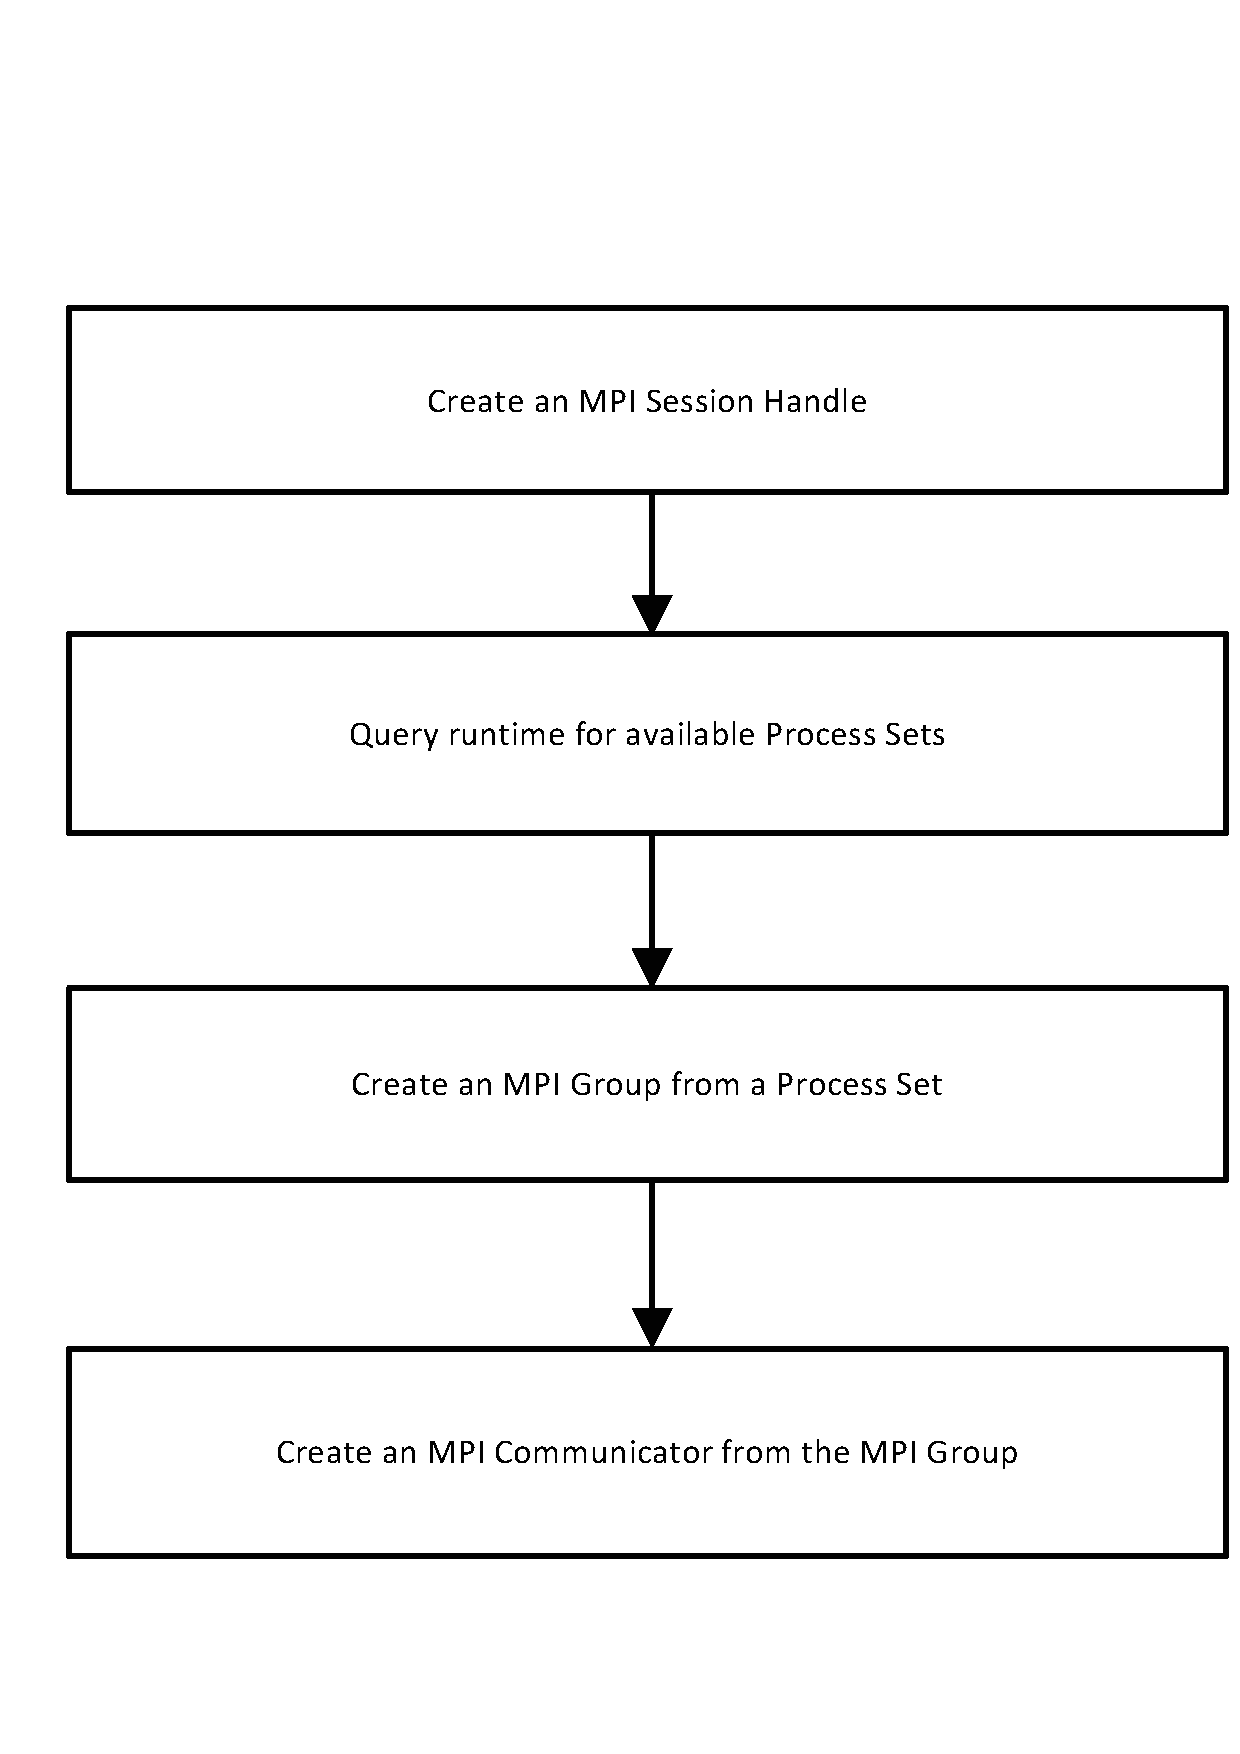
\includegraphics[width=3.50in]{figures/session_flow}}
  \caption[Session handle to communicator]{Steps to creating an \MPI/ Communicator from an \MPI/ Session handle.}
  \label{sessions-fig}
\end{figure}

\subsection{Session Creation and Destruction Methods}
\label{sec:session-init-finalize}

\mpictypemainindex{MPI\_Session}%
\mpictypemainindex{TYPE(MPI\_Session)}%
\begin{mpi-binding}
    function_name("MPI_Session_init")
    parameter("info", "INFO", desc=r"info object to specify thread support level and \MPI/ implementation specific resources")
    parameter("errhandler", "ERRHANDLER", desc=r"error handler to invoke in the event that an error is encountered during this function call")
    parameter("session", "SESSION", direction="OUT", desc=r"new session")
\end{mpi-binding}
%DAN-PyConv%\begin{funcdef}{MPI\_SESSION\_INIT(info, errhandler, session)}
%DAN-PyConv%\funcarg{\IN}{info}{info object to specify thread support level, \MPI/ implementation specific resources, etc. (handle)}
%DAN-PyConv%\funcarg{\IN}{errhandler}{specifies an error handler to invoke in the event that an error is encountered during this function call(handle)}
%DAN-PyConv%\funcarg{\OUT}{session}{session object returned by the call (handle)}
%DAN-PyConv%\end{funcdef}
%DAN-PyConv%\mpibind{MPI\_Session\_init(MPI\_Info~info, MPI\_Errhandler~errhandler, MPI\_Session~*session)}
%DAN-PyConv%\mpifnewbind{MPI\_Session\_init(info, errhandler, session, ierror) \fargs TYPE(MPI\_Info), INTENT(IN) :: info \\ TYPE(MPI\_Errhandler), INTENT(IN) :: errhandler\\ TYPE(MPI\_Session), INTENT(OUT) :: session \\ INTEGER, OPTIONAL, INTENT(OUT) :: ierror}
%DAN-PyConv%\mpifbind{MPI\_SESSION\_INIT(INFO, ERRHANDLER, SESSION, IERROR) \fargs INTEGER INFO, ERRHANDLER, SESSION, IERROR}

\noindent
\mpifunc{MPI\_SESSION\_INIT} is a local procedure.\flushline

The \mpiarg{info} argument is used to request \MPI/ functionality requirements and possible \MPI/ implementation specific capabilities.  The following info keys are predefined:

\begin{description}
\item[\infokey{thread\_level}:] Used to request the thread support level required for \MPI/ objects
derived from the Session.  Allowed values are \infovalmain{MPI\_THREAD\_SINGLE}, \infovalmain{MPI\_THREAD\_FUNNELED}, \infovalmain{MPI\_THREAD\_SERIALIZED}, and \infovalmain{MPI\_THREAD\_MULTIPLE}.  Note that the thread support value is specified by a string rather than the integer
values supplied to \mpifunc{MPI\_INIT\_THREAD}.  The thread support level actually provided by the \MPI/ implementation
can be determined via a subsequent call to \mpifunc{MPI\_SESSION\_GET\_INFO} to return the info object associated with
the Session.  The default thread support level is \MPI/ implementation dependent.
\item[\infokey{mpi\_memory\_alloc\_kinds}:]
Used to request support for memory allocation kinds to be used by the calling \MPI/ process on \MPI/ objects derived from the Session.
See Section~\ref{subsec:mem_alloc_kinds}.
A value for this info key can also be supplied as an argument to an \MPI/ startup mechanism as described in Section~\ref{sec:inquiry-mpiexec}.
\end{description}

The \mpiarg{errhandler} argument specifies an error handler to invoke in the event that the
Session instantiation call encounters an error.
The error handler shall be either a pre-defined error handler (see \sectionref{sec:errorhandler})
or one created using \mpifunc{MPI\_SESSION\_CREATE\_ERRHANDLER}.
Session instantiation is intended to be a lightweight operation.
An \MPI/ process may instantiate multiple Sessions. \mpifunc{MPI\_SESSION\_INIT} is always thread safe; multiple threads
within an application may invoke it concurrently.

\begin{users}
Requesting ``\mpiconst{MPI\_THREAD\_SINGLE}'' thread support level is generally not recommended, because this will conflict with other components of an application requesting higher levels of thread support.
\end{users}

\begin{implementors}
Owing to the restrictions of the \mpiconst{MPI\_THREAD\_SINGLE} thread support level, implementators are discouraged from making this the default thread support level for Sessions.
\end{implementors}


\begin{mpi-binding}
    function_name("MPI_Session_finalize")
    parameter("session", "SESSION", direction="INOUT", desc=r"session to be finalized")
\end{mpi-binding}
%DAN-PyConv%\begin{funcdef}{MPI\_SESSION\_FINALIZE(session)}
%DAN-PyConv%\funcarg{\IN}{session}{session to be finalized (handle)}
%DAN-PyConv%\end{funcdef}
%DAN-PyConv%\mpibind{MPI\_Session\_finalize(MPI\_Session~*session)}
%DAN-PyConv%\mpifnewbind{MPI\_Session\_finalize(session, ierror) \fargs TYPE(MPI\_Session), INTENT(INOUT) :: session \\ INTEGER, OPTIONAL, INTENT(OUT) :: ierror}
%DAN-PyConv%\mpifbind{MPI\_SESSION\_FINALIZE(SESSION, IERROR) \fargs INTEGER SESSION, IERROR}

\noindent
This routine cleans up all \MPI/ state associated with the supplied \mpiarg{session}.
Every instantiated Session must be finalized using \mpifunc{MPI\_SESSION\_FINALIZE}.
The handle \mpiarg{session} is set to \mpiconstmain{MPI\_SESSION\_NULL} by the call.

Before an \MPI/ process invokes \mpifunc{MPI\_SESSION\_FINALIZE}, the process must
perform all \MPI/ calls needed to complete its
involvement in \MPI/ communications: it must locally complete all
\MPI/ operations that it initiated and it must execute matching calls needed to complete \MPI/
communications initiated by other processes.
This means that before calling \mpifunc{MPI\_SESSION\_FINALIZE}, all message handles associated
with this session must be received
(with \mpifunc{MPI\_MRECV}\mpifuncindex{MPI\_IMRECV} or derived procedures)
and all request handles associated with this session must be freed
in the case of nonblocking operations,
and must be inactive or freed in the case of persistent or partitioned operations
(i.e., by calling one of the procedures
\mpifuncindex{MPI\_WAIT}%
\mpifuncindex{MPI\_WAITANY}%
\mpifuncindex{MPI\_WAITSOME}%
\mpifuncindex{MPI\_WAITALL}%
\mpifuncindex{MPI\_TEST}%
\mpifuncindex{MPI\_TESTANY}%
\mpifuncindex{MPI\_TESTSOME}%
\mpifuncindex{MPI\_TESTALL}%
\mpiskipfunc{MPI\_\{TEST$|$WAIT\}\{$|$ANY$|$SOME$|$ALL\}}
or \mpifunc{MPI\_REQUEST\_FREE}).

The call to \mpifunc{MPI\_SESSION\_FINALIZE} does not free objects created by
\MPI/ calls; these objects are freed using
\mpifuncindex{MPI\_COMM\_FREE}%
\mpifuncindex{MPI\_ERRHANDLER\_FREE}%
\mpifuncindex{MPI\_GROUP\_FREE}%
\mpifuncindex{MPI\_INFO\_FREE}%
\mpifuncindex{MPI\_OP\_FREE}%
\mpifuncindex{MPI\_REQUEST\_FREE}%
\mpifuncindex{MPI\_TYPE\_FREE}%
\mpifuncindex{MPI\_WIN\_FREE}%
\mpiskipfunc{MPI\_\XXX/\_FREE},
\mpifunc{MPI\_COMM\_DISCONNECT}, or
\mpifunc{MPI\_FILE\_CLOSE} calls.

Once \mpifunc{MPI\_SESSION\_FINALIZE} returns, no \MPI/ procedure may be called in the \spm{} that are related to this session
(not even freeing objects that are derived from this session),
except for those listed in \sectionref{subsec:dynamic:preinit_functions}.

\begin{users}
Opaque objects and their handles may bind internal resources.
Therefore, it is highly recommended to explicitly free the handles associated with this session before finalizing it.
Such associated handles can be group, communicator, window, file, message, and request handles,
whereas datatype, operation (e.g., for reductions), error handler, and info handles exist independently
of the \wpm{} or a session in the \spm{}.
In addition, if attributes are cached on such an opaque object (see \sectionref{sec:caching}),
then the delete callback functions are only invoked when the object is explicitly freed (or disconnected).
\end{users}

Most handles that exist independently from the \wpm{} or a session in the \spm{}, e.g., datatype handles,
can be created only while \MPI/ is initialized.
For example, a datatype handle that was created when one particular session existed
can be used in any other session (or in the \wpm{}), even if the second session
was initialized after the first session had already been finalized
and no other session existed in between.
See \sectionref{subsec:dynamic:preinit_functions} for handle creation procedures that do not require that \MPI/ is initialized.

\mpifunc{MPI\_SESSION\_FINALIZE} may be synchronizing on any or all of the groups associated with
communicators, windows, or files derived from the session and not disconnected, freed, or closed,
respectively, before the call to the \mpifunc{MPI\_SESSION\_FINALIZE} procedure.
\mpifunc{MPI\_SESSION\_FINALIZE} behaves as if all such synchronizations occur concurrently.
As \mpifunc{MPI\_COMM\_FREE} may mark a communicator for freeing later,
\mpifunc{MPI\_SESSION\_FINALIZE} may be synchronizing on the group associated
with a communicator that is only freed (with \mpifunc{MPI\_COMM\_FREE})
rather than disconnected (with \mpifunc{MPI\_COMM\_DISCONNECT}).

\begin{rationale}
This rule is similar to the rule that \mpifunc{MPI\_FINALIZE} is collective (see \sectionref{sec:inquiry-finalize}),
but does not require that \mpifunc{MPI\_SESSION\_FINALIZE} be collective over all connected \MPI/ processes.
It also allows for cases where some \MPI/ processes may have derived a set of communicators
using a different number of session handles.  See Example~\ref{exa:session_finalize}.
\end{rationale}

\begin{implementors}
This rule also allows for the completion of communications the \MPI/ process is involved with
that may not yet be completed from the viewpoint of the underlying \MPI/ system.
See \sectionref{subsec:terms:progress} on \mpitermni{progress}\mpitermindex{progress!finalize!session}
and the advice to implementors at the end of Section~\ref{sec:inquiry-finalize}.
\end{implementors}

\begin{implementors}
An \MPI/ implementation should be able to implement the semantics of \mpifunc{MPI\_SESSION\_FINALIZE}
as a \mpiterm{local} procedure,
provided an application frees all \MPI/ windows, closes all \MPI/ files,
and uses \mpifunc{MPI\_COMM\_DISCONNECT} to free all \MPI/ communicators
associated with a session
prior to invoking \mpifunc{MPI\_SESSION\_FINALIZE} on the corresponding session handle.
\end{implementors}

\begin{example}
\label{exa:session_finalize}
\Exindex{Neutral}{Finalize in the Sessions Model}{MPI\_SESSION\_FINALIZE}
Three \MPI/ processes are connected with 2 communicators (indicated by the \code{=} symbols),
derived from one session handle in process X but from two separate session handles
in both process Y and Z.
%%HEADER
%%SKIP
%%ENDHEADER
\begin{verbatim}
  process-X     process-Y     process-Z     Remarks
                                            sesX, sesYA, sesYB, sesZA and
                                              sesZB are session handles.
    (sesX)=======(sesYA)=======(sesZA)      communicator_1 and
    (sesX)=======(sesYB)=======(sesZB)      communicator_2 are derived
                                              from them.
   SF(sesX)     SF(sesYA)     SF(sesZA)     SF = MPI_SESSION_FINALIZE
                SF(sesYB)     SF(sesZB)
\end{verbatim}

Process X has only to finalize its one session handle,
whereas the other two \MPI/ processes have to call
\mpifunc{MPI\_SESSION\_FINALIZE} twice in the same sequence with respect to
the communicators derived from the session handles.
Specifically, both process Y and process Z shall call \mpifunc{MPI\_SESSION\_FINALIZE}
for the session from which \code{communicator\_1} was derived before calling the
\mpifunc{MPI\_SESSION\_FINALIZE} for the session from which \code{communicator\_2} was derived,
or vice versa (i.e., both shall finalize the session for \code{communicator\_2}
first then finalize the session for \code{communicator\_1}).
The call \code{SF(sesX)} in process X may not return until
both \code{SF(ses*A)} and \code{SF(ses*B)} are called in processes Y and Z.
\end{example}

\subsection{Processes Sets}
\label{subsec:process_sets}

Process sets are the mechanism for \MPI/ applications to query the runtime.
Process sets are identified by process set names.
Process set names have a \emph{Uniform Resource Identifier}~(URI) format.
Two process set names are mandated: \mpistringmain{mpi://WORLD} and \mpistringmain{mpi://SELF}.
Additional process set names may be defined,
for example, \mpistringskip{mpix://UNIVERSE} and \mpistringskip{hwloc://L3Cache}
may be defined by the \MPI/ implementation.
The \mpistring{mpi://} namespace is reserved for exclusive use by the \MPI/ standard.
Figure~\ref{sessions-pset-fig} depicts process sets that the runtime could associate with an instance of an \MPI/ job.
In this example, the two mandated process sets are defined, in addition to optional, implementation specific ones.

Mechanisms for defining process sets and how system resources are assigned to these sets
is considered to be implementation dependent.

A process set caches (\mpiarg{key},\mpiarg{value}) pairs that are accessible to the application via an \mpictype{MPI\_Info} object.
The \infokey{mpi\_size} key is mandatory for all process sets.

\begin{figure}
  \centerline{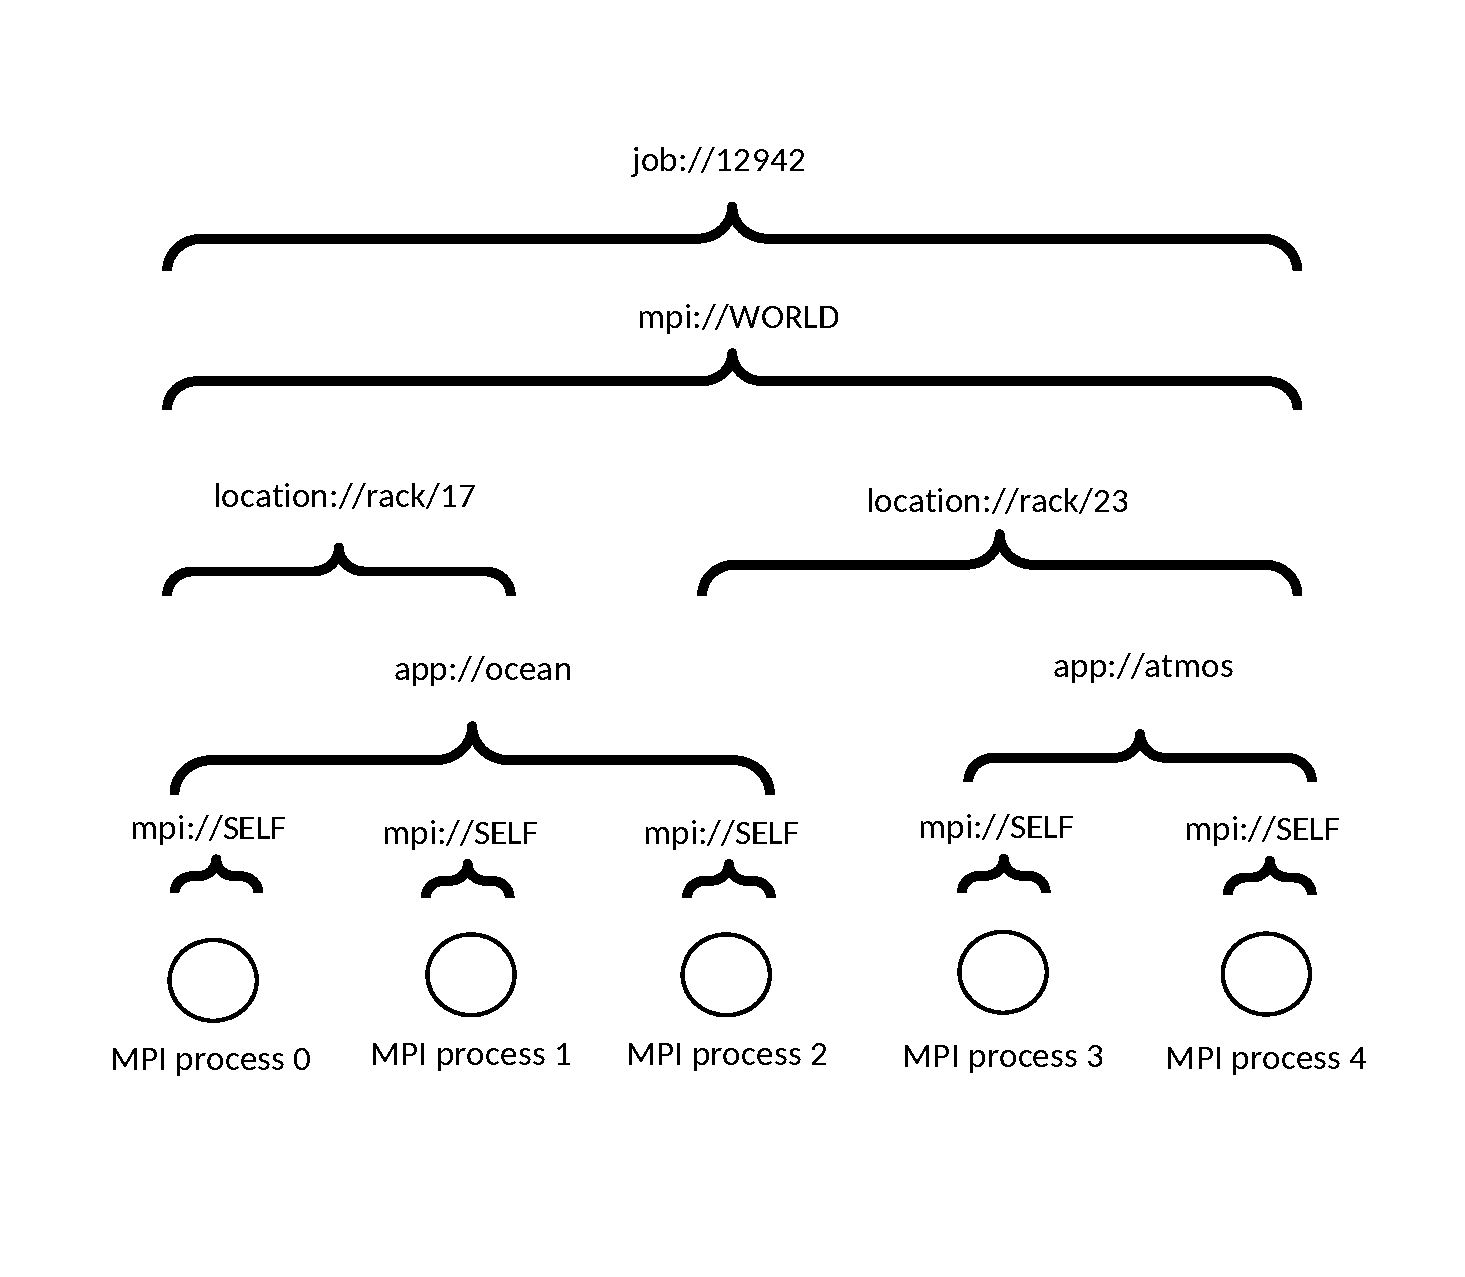
\includegraphics[width=4.50in]{figures/figure_pset}}
  \caption[Process set examples]{Examples of process sets.  Illustrated are the two mandated process sets---\mpistring{mpi://WORLD} and \mpistring{mpi://SELF}---along with several optional ones that a runtime could define.  In this example, \mpifunc{MPI\_SESSION\_GET\_NUM\_PSETS} would return five at each \MPI/ process. }
  \label{sessions-pset-fig}
\end{figure}

\subsection{Runtime Query Functions}

\begin{mpi-binding}
    function_name("MPI_Session_get_num_psets")
    parameter("session", "SESSION", desc=r"session")
    parameter("info", "INFO", desc=r"info object")
    parameter("npset_names", "ARRAY_LENGTH_NNI", direction="OUT", desc=r"number of available process sets")
\end{mpi-binding}
%DAN-PyConv%\begin{funcdef}{MPI\_SESSION\_GET\_NUM\_PSETS(session, info, npset\_names)}
%DAN-PyConv%\funcarg{\IN}{session}{session (handle)}
%DAN-PyConv%\funcarg{\IN}{info}{info object (handle)}
%DAN-PyConv%\funcarg{\OUT}{npset\_names}{number of available process sets}
%DAN-PyConv%\end{funcdef}
%DAN-PyConv%\mpibind{MPI\_Session\_get\_num\_psets(MPI\_Session~session, MPI\_Info~info, int~*npset\_names)}
%DAN-PyConv%\mpifnewbind{MPI\_Session\_get\_num\_psets(session, info, npset\_names, ierror) \fargs TYPE(MPI\_Session), INTENT(IN) :: session \\ TYPE(MPI\_Info), INTENT(IN) :: info \\ INTEGER, INTENT(OUT) :: npset\_names \\ INTEGER, OPTIONAL, INTENT(OUT) :: ierror}
%DAN-PyConv%\mpifbind{MPI\_SESSION\_GET\_NUM\_PSETS(SESSION, INFO, NPSET\_NAMES, IERROR) \fargs INTEGER SESSION, INFO, NPSET\_NAMES, IERROR}

This function is used to query the runtime for the number of available process sets in which the calling \MPI/ process is a member.
An \MPI/ implementation is allowed to increase the number of available process sets
during the execution of an \MPI/ application when new process sets become available.
However, \MPI/ implementations are not allowed
to change the index of a particular process set name,
or to change the name of the process set at a particular index,
or to delete a process set name once it has been added.
When a process set becomes invalid,
for example, when some processes become unreachable due to failures in the communication system,
subsequent usage of the process set name should raise an error.
For example, creating an \mpictype{MPI\_Group} from such a process set might succeed because it is a local operation,
but creating an \mpictype{MPI\_Comm} from that group and attempting collective communication
should raise an error.

\begin{implementors}
It is anticipated that an \MPI/ implementation may be relying on an external runtime system to provide process sets.
Such runtime systems may have the ability to dynamically create process sets during the course of application execution.
Requiring the number of process sets returned by \mpifunc{MPI\_SESSION\_GET\_NUM\_PSETS}
to be constant over the course of application execution would prevent an application from taking advantage of such capabilities.
\end{implementors}

\begin{mpi-binding}
    function_name("MPI_Session_get_nth_pset")
    parameter("session", "SESSION", desc=r"session")
    parameter("info", "INFO", desc=r"info object")
    parameter("n", "INDEX", desc=r"index of the desired process set name")
    parameter("pset_len", "STRING_LENGTH", direction="INOUT", desc=r"length of the pset\_name argument")
    parameter("pset_name", "STRING", direction="OUT", desc=r"name of the \mpiarg{n}th process set")
\end{mpi-binding}
%DAN-PyConv%\begin{funcdef}{MPI\_SESSION\_GET\_NTH\_PSET(session, info, n, pset\_len, pset\_name)}
%DAN-PyConv%\funcarg{\IN}{session}{session (handle)}
%DAN-PyConv%\funcarg{\IN}{info}{info object (handle)}
%DAN-PyConv%\funcarg{\IN}{n}{process set name number (integer)}
%DAN-PyConv%\funcarg{\INOUT}{pset\_len}{length of the pset\_name argument}
%DAN-PyConv%\funcarg{\OUT}{pset\_name}{pset\_name (string)}
%DAN-PyConv%\end{funcdef}
%DAN-PyConv%\mpibind{MPI\_Session\_get\_nth\_pset(MPI\_Session~session, MPI\_Info~info, int~n, int~*pset\_len, char~*pset\_name)}
%DAN-PyConv%\mpifnewbind{MPI\_Session\_get\_nth\_pset(session, info, n, pset\_len, pset\_name, ierror) \fargs TYPE(MPI\_Session), INTENT(IN) :: session \\ TYPE(MPI\_Info), INTENT(IN) :: info \\ INTEGER, INTENT(IN) :: n \\ INTEGER, INTENT(INOUT) :: pset\_len \\ CHARACTER(LEN=pset\_len), INTENT(OUT) :: pset\_name \\ INTEGER, OPTIONAL, INTENT(OUT) :: ierror}
%DAN-PyConv%\mpifbind{MPI\_SESSION\_GET\_NTH\_PSET(SESSION, INFO, N, PSET\_LEN, PSET\_NAME, IERROR)\fargs INTEGER SESSION, INFO, PSET\_LEN, IERROR \\CHARACTER*(*) PSET\_NAME}

This function returns the name of the \mpiarg{n}th process set in the supplied \mpiarg{pset\_name} buffer.
\mpiarg{pset\_len} is the size of the buffer needed to store the \mpiarg{n}th process set name.  If the \mpiarg{pset\_len} passed
into the function is less than the actual buffer size needed for the process set name,
then the string value returned in \mpiarg{pset\_name} is truncated.
If \mpiarg{pset\_len} is set to 0, \mpiarg{pset\_name} is not changed.  On return, the value of \mpiarg{pset\_len} will be set
to the required buffer size to hold the process set name.  In C, \mpiarg{pset\_len} includes the required space for the null terminator.
In C, this function returns a null terminated string in all cases where the \mpiarg{pset\_len} input value is greater than 0.

If two \MPI/ processes get the same process set name, then the intersection of the two process sets shall either be the empty set or identical to the union of the two process sets.

After a successful call to \mpifunc{MPI\_SESSION\_GET\_NTH\_PSET}, subsequent calls to routines that query information about the same process set name and same session handle must return the same information. An \MPI/ implementation is not allowed to alter any of the returned process set names.

Process set names have an implementation-defined maximum length of \mpiconst{MPI\_MAX\_PSET\_NAME\_LEN} characters.  \mpiconstmain{MPI\_MAX\_PSET\_NAME\_LEN} shall have a value of at least 63.

\begin{users}
\mpiconst{MPI\_MAX\_PSET\_NAME\_LEN} might be very large, so it
might not be wise to declare a string of that size.
Users are encouraged to use \mpifunc{MPI\_SESSION\_GET\_NTH\_PSET}
both for obtaining the length of a \mpiarg{pset\_name} and the process set name.
\end{users}

\begin{mpi-binding}
    function_name("MPI_Session_get_info")
    parameter("session", "SESSION", desc=r"session")
    parameter("info_used", "INFO", direction="OUT", desc=r"see explanation below")
\end{mpi-binding}
%DAN-PyConv%\begin{funcdef}{MPI\_SESSION\_GET\_INFO(session, info\_used)}
%DAN-PyConv%\funcarg{\IN}{session}{session (handle)}
%DAN-PyConv%\funcarg{\OUT}{info\_used}{see explanation below (handle)}
%DAN-PyConv%\end{funcdef}
%DAN-PyConv%\mpibind{MPI\_Session\_get\_info(MPI\_Session~session, MPI\_Info~*info\_used)}
%DAN-PyConv%\mpifnewbind{MPI\_Session\_get\_info(session, info\_used, ierror) \fargs TYPE(MPI\_Session), INTENT(IN) :: session \\ TYPE(MPI\_Info), INTENT(OUT) :: info\\ INTEGER, OPTIONAL, INTENT(OUT) :: ierror}
%DAN-PyConv%\mpifbind{MPI\_SESSION\_GET\_INFO(SESSION, INFO\_USED, IERROR) \fargs INTEGER SESSION, INFO\_USED, IERROR}

\mpifunc{MPI\_SESSION\_GET\_INFO} returns a new info object containing
the hints of the \MPI/ Session  associated with \mpiarg{session}.
The current setting of all hints related to this \MPI/ Session is
returned in \mpiarg{info\_used}.  An \MPI/ implementation is required to
return all hints that are supported by the implementation and have
default values specified; any user-supplied hints that were not ignored
by the implementation; and any additional hints that were set by
the implementation.
If no such hints
exist, a handle to a newly created info object is returned that
contains no key/value pair.
The user is responsible for freeing
\mpiarg{info\_used} via \mpifunc{MPI\_INFO\_FREE}.

\begin{mpi-binding}
    function_name("MPI_Session_get_pset_info")
    parameter("session", "SESSION", desc=r"session")
    parameter("pset_name", "STRING", constant=True, desc=r"name of process set")
    parameter("info", "INFO", direction="OUT", desc=r"info object containing information about the given process set")
\end{mpi-binding}
%DAN-PyConv%\begin{funcdef}{MPI\_SESSION\_GET\_PSET\_INFO(session, pset\_name, info)}
%DAN-PyConv%\funcarg{\IN}{session}{session (handle)}
%DAN-PyConv%\funcarg{\IN}{set\_name}{name of process set to query}
%DAN-PyConv%\funcarg{\OUT}{info}{info object containing information about the given process set (handle)}
%DAN-PyConv%\end{funcdef}
%DAN-PyConv%\mpibind{MPI\_Session\_get\_pset\_info(MPI\_Session~session, char~*pset\_name, MPI\_Info~*info)}
%DAN-PyConv%\mpifnewbind{MPI\_Session\_get\_pset\_info(session, set\_name, info, ierror) \fargs TYPE(MPI\_Session), INTENT(IN) :: session \\ CHARACTER(len=*), INTENT(IN) :: pset\_name \\ TYPE(MPI\_Info), INTENT(OUT) :: info\\ INTEGER, OPTIONAL, INTENT(OUT) :: ierror}
%DAN-PyConv%\mpifbind{MPI\_SESSION\_GET\_PSET\_INFO(SESSION, PSET\_NAME, INFO, IERROR) \fargs INTEGER SESSION, INFO, IERROR \\ CHARACTER(*) PSET\_NAME}

This function is used to query properties of a specific process set.
The returned \mpiarg{info} object can be queried with existing \MPI/ info object query functions.
One key/value pair must be defined, \infokey{mpi\_size}.
The value of the \infokeymain{mpi\_size} key specifies the number of \MPI/ processes in the process set.
The user is responsible for freeing the returned \mpictype{MPI\_Info} object.

\subsection{\texorpdfstring{\spm}{Sessions Model} Examples}

This section presents several examples of how to use \MPI/ Sessions to create \MPI/ Groups and \MPI/ Communicators.

\begin{example}
Example illustrating creation of an \MPI/ communicator using the \spm{}.
\label{exa:session1}
\Exindex{C}{Creating a communicator using the \spm}{MPI\_Session\_init,MPI\_Info\_create,MPI\_Info\_set,MPI\_Session\_finalize,MPI\_Group\_from\_session\_pset,MPI\_Comm\_create\_from\_group}%
%%HEADER
%%LANG: C
%%ENDHEADER
\begin{lstlisting}[language={[MPI]C}]
#include <stdio.h>
#include <stdlib.h>
#include <string.h>
#include "mpi.h"

static MPI_Session lib_shandle = MPI_SESSION_NULL;
static MPI_Comm lib_comm = MPI_COMM_NULL;

int library_foo_init(void)
{
   int rc, flag, valuelen;
   int ret = 0;
   const char pset_name[] = "mpi://WORLD";
   const char mt_key[] = "thread_level";
   const char mt_value[] = "MPI_THREAD_MULTIPLE";
   char out_value[100];   /* large enough */
   MPI_Group wgroup = MPI_GROUP_NULL;
   MPI_Info sinfo = MPI_INFO_NULL;
   MPI_Info tinfo = MPI_INFO_NULL;

   MPI_Info_create(&sinfo);
   MPI_Info_set(sinfo, mt_key, mt_value);
   rc = MPI_Session_init(sinfo, MPI_ERRORS_RETURN,
                         &lib_shandle);
   if (rc != MPI_SUCCESS) {
      ret = -1;
      goto fn_exit;
   }

   /*
    * check we got thread support level foo library needs
    */
   rc = MPI_Session_get_info(lib_shandle, &tinfo);
   if (rc != MPI_SUCCESS) {
      ret = -1;
      goto fn_exit;
   }

   valuelen = sizeof(out_value);
   MPI_Info_get_string(tinfo, mt_key, &valuelen,
                       out_value, &flag);
   if (0 == flag) {
      printf("Could not find key %s\n", mt_key);
      ret = -1;
      goto fn_exit;
   }

   if (strcmp(out_value, mt_value)) {
      printf("Did not get thread multiple support, got %s\n",
             out_value);
      ret = -1;
      goto fn_exit;
   }

   /*
    * create a group from the WORLD process set
    */
   rc = MPI_Group_from_session_pset(lib_shandle,
                                    pset_name,
                                    &wgroup);
   if (rc != MPI_SUCCESS) {
      ret = -1;
      goto fn_exit;
   }

   /*
    * get a communicator
    */
   rc = MPI_Comm_create_from_group(wgroup,
                              "org.mpi-forum.mpi-v4_0.example-ex11_10",
                              MPI_INFO_NULL,
                              MPI_ERRORS_RETURN,
                              &lib_comm);
   if (rc != MPI_SUCCESS) {
      ret = -1;
      goto fn_exit;
   }

   /*
    * release unused resources
    */

fn_exit:
   if (wgroup != MPI_GROUP_NULL) {
      MPI_Group_free(&wgroup);
   }

   if (sinfo != MPI_INFO_NULL) {
      MPI_Info_free(&sinfo);
   }

   if (tinfo != MPI_INFO_NULL) {
      MPI_Info_free(&tinfo);
   }

   if (ret != 0) {
      MPI_Session_finalize(&lib_shandle);
   }

   return ret;
}
\end{lstlisting}
\end{example}

Example~\ref{exa:session1} shows how the predefined \mpistring{mpi://WORLD} process set can be used to
first create a local \MPI/ group and then subsequently to create an \MPI/ communicator from this
group. 

\begin{example}
This example illustrates the use of Process Set query functions
to select a Process Set to use for \MPI/ Group creation.
\label{exa:session2}
\Exindex{C}{Using process set query in group creation}{MPI\_Session\_init,MPI\_Session\_finalize,MPI\_Group\_from\_session\_pset,MPI\_Session\_get\_num\_psets,MPI\_Session\_get\_nth\_pset}%
%%HEADER
%%LANG: C
%%ENDHEADER
\begin{lstlisting}[language={[MPI]C},basicstyle=\lstsmall]
#include <stdio.h>
#include <stdlib.h>
#include <string.h>
#include "mpi.h"

int main(int argc, char *argv[])
{
   int i, n_psets, psetlen, rc, ret;
   int valuelen;
   int flag = 0;
   char *pset_name = NULL;
   char *info_val = NULL;
   MPI_Session shandle = MPI_SESSION_NULL;
   MPI_Info sinfo = MPI_INFO_NULL;
   MPI_Group pgroup = MPI_GROUP_NULL;

   if (argc < 2) {
      fprintf(stderr, "A process set name fragment is required\n");
      return EXIT_FAILURE;
   }

   rc = MPI_Session_init(MPI_INFO_NULL, MPI_ERRORS_RETURN, &shandle);
   if (rc != MPI_SUCCESS) {
      fprintf(stderr, "Could not initialize session, bailing out\n");
      return EXIT_FAILURE;
   }

   MPI_Session_get_num_psets(shandle, MPI_INFO_NULL, &n_psets);

   for (i=0, pset_name=NULL; i<n_psets; i++) {
       psetlen = 0;
       MPI_Session_get_nth_pset(shandle, MPI_INFO_NULL, i,
                                &psetlen, NULL);
       pset_name = (char *)malloc(sizeof(char) * psetlen);
       MPI_Session_get_nth_pset(shandle, MPI_INFO_NULL, i,
                                &psetlen, pset_name);
       if (strstr(pset_name, argv[1]) != NULL) break;

       free(pset_name);
       pset_name = NULL;
   }

   if (pset_name == NULL) {
       fprintf(stderr, "Unable to find matching process set\n");
       return EXIT_FAILURE;
   }

   /*
    * get instance of an info object for this Session
    */

   MPI_Session_get_pset_info(shandle, pset_name, &sinfo);
   valuelen = 0;
   MPI_Info_get_string(sinfo, "mpi_size", &valuelen, NULL, &flag);
   if (flag) {
       info_val = (char *)malloc(valuelen);
       MPI_Info_get_string(sinfo, "mpi_size", &valuelen, info_val, &flag);
       free(info_val);
    }

   /*
    * create a group from the process set
    */

   rc = MPI_Group_from_session_pset(shandle, pset_name,
                                    &pgroup);
   ret = (rc == MPI_SUCCESS) ? 0 : EXIT_FAILURE;

   free(pset_name);
   if (pgroup != MPI_GROUP_NULL) {
       MPI_Group_free(&pgroup);
   }
   MPI_Info_free(&sinfo);
   MPI_Session_finalize(&shandle);

   fprintf(stderr, "Test completed ret = %d\n", ret);
   return ret;
}
\end{lstlisting}
\end{example}

Example~\ref{exa:session2} illustrates several aspects of the \spm{}. First, the default error handler
can be specified when instantiating a Session instance.  Second, there must be at least two process sets
associated with a Session.  Third, the example illustrates use of the Sessions info object and the
one required key: \infokey{mpi\_size}.


\begin{example}
A Fortran 2008 example illustrating how to obtain information about available process sets, create an \MPI/ Group
from a process set, and subsequently create an \MPI/ Communicator.
\label{exa:session3}
\Exindex{Fortran}{Using process set query in group creation}{MPI\_Session\_init,MPI\_Session\_finalize,MPI\_Group\_from\_session\_pset,MPI\_Comm\_create\_from\_group,MPI\_Barrier,MPI\_Session\_get\_num\_psets,MPI\_Session\_get\_nth\_pset}%
%%HEADER
%%LANG: FORTRAN08
%%ENDHEADER
\begin{lstlisting}[language={[MPI08withlen]Fortran},basicstyle=\lstsmall]
PROGRAM MAIN
    USE mpi_f08
    IMPLICIT NONE
    INTEGER :: pset_len, ierror, n_psets
    CHARACTER(LEN=:), ALLOCATABLE :: pset_name
    TYPE(MPI_Session) :: shandle
    TYPE(MPI_Group) :: pgroup
    TYPE(MPI_Comm) :: pcomm

    CALL MPI_Session_init(MPI_INFO_NULL, MPI_ERRORS_RETURN, &
                         shandle, ierror)
    IF (ierror .NE. MPI_SUCCESS) THEN
       WRITE(*,*) "MPI_Session_init failed"
       ERROR STOP
    END IF

    CALL MPI_Session_get_num_psets(shandle, MPI_INFO_NULL, n_psets)
    IF (n_psets .LT. 2)  THEN
       WRITE(*,*) "MPI_Session_get_num_psets didn't return at least 2 psets"
       ERROR STOP
    END IF

!
!   Just get the second pset's length and name
!   Note that index values are zero-based, even in Fortran
!

    pset_len = 0
    CALL MPI_Session_get_nth_pset(shandle, MPI_INFO_NULL, 1,     &
                                  pset_len, pset_name)
    ALLOCATE(CHARACTER(LEN=pset_len)::pset_name)
    CALL MPI_Session_get_nth_pset(shandle, MPI_INFO_NULL, 1,     &
                                  pset_len, pset_name)

!
!   create a group from the pset
!
    CALL MPI_Group_from_session_pset(shandle, pset_name, pgroup)
!
!   free the buffer used for the pset name
!
    DEALLOCATE(pset_name)

!
!   create a MPI communicator from the group
!
    CALL MPI_Comm_create_from_group(pgroup, "session_example",    &
                                    MPI_INFO_NULL,                &
                                    MPI_ERRORS_RETURN,            &
                                    pcomm)

    CALL MPI_Barrier(pcomm, ierror)
    IF (ierror .NE. MPI_SUCCESS) THEN
        WRITE(*,*) "Barrier call on communicator failed"
        ERROR STOP
    END IF

    CALL MPI_Comm_free(pcomm)
    CALL MPI_Group_free(pgroup)
    CALL MPI_Session_finalize(shandle, ierror)

END PROGRAM MAIN
\end{lstlisting}
\end{example}

Note in this example that the call to \mpifunc{MPI\_SESSION\_FINALIZE} may block in order to
ensure that the calling \MPI/ process has completed its involvement in the preceding \mpifunc{MPI\_BARRIER} operation.  If \mpifunc{MPI\_COMM\_DISCONNECT} had been used instead of \mpifunc{MPI\_COMM\_FREE}, the example would have blocked in \mpifunc{MPI\_COMM\_DISCONNECT} rather than \mpifunc{MPI\_SESSION\_FINALIZE}.


\section{Common Elements of Both Process Models}
\label{sec:dynamic:common-elements}

\subsection{\texorpdfstring{\MPI/}{MPI} Functionality that is Always Available}
\label{subsec:dynamic:preinit_functions}

Some \MPI/ functions may be invoked
at any time, including
prior to calling \mpifunc{MPI\_INIT} or \mpifunc{MPI\_SESSION\_INIT},
and following \MPI/ finalization,
independent of whether the \wpm{}, \spm{}, or both are used.
These functions can be called concurrently by multiple threads within an \MPI/ Process.
Table~\ref{table:dynamic:preinit_functions} lists the applicable \MPI/ functions.

\begin{table}[t!]
\caption{List of \MPI/ Functions
that can be called at any time within an \MPI/ program, including
prior to \MPI/ initialization and following \MPI/ finalization}
\label{table:dynamic:preinit_functions}
\begin{center}
\begin{tabular}{|l|}
\hline
\mpifunc{MPI\_INITIALIZED}  \\
\mpifunc{MPI\_FINALIZED}  \\
\hline
\mpifunc{MPI\_GET\_VERSION} \\
\mpifunc{MPI\_GET\_LIBRARY\_VERSION} \\
\hline
\mpifunc{MPI\_ABI\_GET\_VERSION} \\
\mpifunc{MPI\_ABI\_GET\_INFO} \\
\hline
\mpifunc{MPI\_INFO\_CREATE} \\
\mpifunc{MPI\_INFO\_CREATE\_ENV} \\
\mpifunc{MPI\_INFO\_SET} \\
\mpifunc{MPI\_INFO\_DELETE} \\
\mpifunc{MPI\_INFO\_GET\_STRING} \\
\mpifunc{MPI\_INFO\_GET\_NKEYS} \\
\mpifunc{MPI\_INFO\_GET\_NTHKEY} \\
\mpifunc{MPI\_INFO\_DUP} \\
\mpifunc{MPI\_INFO\_FREE} \\
\hline
\mpifunc{MPI\_INFO\_F2C} \\
\mpifunc{MPI\_INFO\_C2F} \\
\hline
\mpifunc{MPI\_SESSION\_CREATE\_ERRHANDLER} \\
\mpifunc{MPI\_SESSION\_CALL\_ERRHANDLER}\\
\hline
\mpifunc{MPI\_ERRHANDLER\_FREE} \\
\mpifunc{MPI\_ERRHANDLER\_F2C} \\
\mpifunc{MPI\_ERRHANDLER\_C2F} \\
\mpifunc{MPI\_ERROR\_STRING} \\
\mpifunc{MPI\_ERROR\_CLASS} \\
\mpifunc{MPI\_ADD\_ERROR\_CLASS} \\
\mpifunc{MPI\_REMOVE\_ERROR\_CLASS} \\
\mpifunc{MPI\_ADD\_ERROR\_CODE} \\
\mpifunc{MPI\_REMOVE\_ERROR\_CODE} \\
\mpifunc{MPI\_ADD\_ERROR\_STRING} \\
\mpifunc{MPI\_REMOVE\_ERROR\_STRING} \\
\hline
\end{tabular}
\end{center}
\end{table}

In addition to the functions listed in Table~\ref{table:dynamic:preinit_functions}, any function with the prefix \mpicode{MPI\_T\_} (within the constraints for functions with this prefix listed in Section~\ref{sec:mpit:init}) may also be called prior to \MPI/ initialization and after \MPI/ finalization.

\subsection{Aborting \texorpdfstring{\mpi/}{MPI} Processes}

\begin{mpi-binding}
    function_name("MPI_Abort")
    parameter(
        "comm",
        "COMMUNICATOR",
        desc=r"communicator of \MPI/ processes to abort",
    )
    parameter(
        "errorcode",
        "ERROR_CODE",
        desc=r"error code to return to invoking environment",
    )
\end{mpi-binding}

This routine makes a ``best attempt'' to abort all \MPI/ processes in the group
of \mpiarg{comm}.
This function does not require that the invoking environment take any action
with the error code.  However, a Unix or POSIX environment should handle this
as a \code{return errorcode} from the main program.


It may not be possible for an \MPI/ implementation to abort only the
processes represented by \mpiarg{comm} if this is a subset of the processes.
In this case, the \MPI/ implementation should attempt to abort all the connected
processes but should not abort any unconnected processes.
When using the \wpm{}, and
if no processes were spawned, accepted, or connected then this has the effect
of aborting all the processes associated with \mpiconst{MPI\_COMM\_WORLD}.
In the case of the \spm{}, if an \MPI/ process
has instantiated multiple sessions, the union of the process sets in these
sessions are considered connected processes.  Thus invoking \mpifunc{MPI\_ABORT} on
a communicator derived from one of these sessions will result in all \MPI/ processes
in this union being aborted.

\begin{implementors}
    After aborting a subset of processes, a high-quality implementation should
    be able to provide error handling for communicators, windows, and files
    involving both aborted and nonaborted processes. As an example, if the
    user changes the error handler for \mpiconst{MPI\_COMM\_WORLD} to
    \mpiconst{MPI\_ERRORS\_RETURN} or a custom error handler, when a subset of
    \mpiconst{MPI\_COMM\_WORLD} is aborted, the remaining processes in
    \mpiconst{MPI\_COMM\_WORLD} should be able to continue communicating with each
    other and receive an appropriate error code when attempting communication
    with an aborted process (e.g., an error of class \errormain{MPI\_ERR\_PROC\_ABORTED}).
    A high-quality implementation should support
    equivalent behavior for communicators derived from sessions.
\end{implementors}

\begin{users}
Whether the \mpiarg{errorcode} is returned from the executable or from the
\MPI/ process startup mechanism (e.g., \mpilaunch{mpiexec}), is an aspect of quality
of the \MPI/ library but not mandatory.
\end{users}
\begin{implementors}
Where possible, a high-quality implementation will try to return the
\mpiarg{errorcode} from the \MPI/ process startup mechanism
(e.g. \mpilaunch{mpiexec} or singleton init).
\end{implementors}

\subsection{Memory Allocation Info}
\label{subsec:mem_alloc_kinds}

Computing systems contain memory with different properties, including differences in
performance, persistence, access permissions, or access mode.
These distinct memories are generally allocated using distinct mechanisms and are
referred to as memory allocation kinds that are named according to the method of allocation.
The following info keys can be used to request or query the memory allocation
kinds supported by the \MPI/ library and to assert application usage of memory
allocation kinds with respect to specific \MPI/ objects, as shown in Example~\ref{example:alloc-kinds-spm}.

\begin{description}

{\sloppy %%ALLOWLATEX% to avoid overfull line
\item[\infokeymain{mpi\_memory\_alloc\_kinds} (string, default: \infovalskip{mpi,system}):]
A comma-separated list of memory allocation kinds. When defaulted, the value returned
must, at minimum, contain the kinds specified in \infovalmain{default} and may contain
additional implementation-defined kinds. Different sessions may return different default
values.

When set on the input info object in a call to
        \mpifunc{MPI\_SESSION\_INIT},
        \mpifunc{MPI\_COMM\_SPAWN},
        or \mpifunc{MPI\_COMM\_SPAWN\_MULTIPLE},
or when supplied as an argument to an \MPI/ startup mechanism, this info key
requests support for the specified memory allocation kinds.

}
%
When returned by \MPI/, this info key indicates the memory allocation kinds
supported by the \MPI/ library on the given session, \MPI/ object, or objects
derived from the \wpm{}.
%
This info key does not affect the kind of memory allocated by \MPI/, e.g., in a
call to \mpifunc{MPI\_ALLOC\_MEM} or \mpifunc{MPI\_WIN\_ALLOCATE}.
%
A value corresponding to the empty string represents no memory allocation kinds.

\item[\infokeymain{mpi\_assert\_memory\_alloc\_kinds} (string, not set by default):]
A comma separated list of memory allocation kinds that the calling \MPI/ process will
use with the given \MPI/ object.
%
A value corresponding to the empty string represents no memory allocation kinds.

\end{description}

The \infokey{mpi\_memory\_alloc\_kinds} info key is used both for requesting
and querying support for memory allocation kinds from the \MPI/ library.

When supplied to \mpifunc{MPI\_SESSION\_INIT}, this info key requests support
for memory allocation kinds for all objects that will be derived from the new
session.
%
This info hint can also be supplied through an argument to an \MPI/ startup mechanism.
%
In the \spm{}, this behaves as though the \infokey{mpi\_memory\_alloc\_kinds}
info key with the given value was supplied in the info argument in calls to
\mpifunc{MPI\_SESSION\_INIT}.
%
A value of \infokey{mpi\_memory\_alloc\_kinds} supplied in the info argument to
\mpifunc{MPI\_SESSION\_INIT} takes precedence over a value supplied as an
argument to an \MPI/ startup mechanism.

In the \wpm{}, an info hint passed to an \MPI/ startup mechanism requests support for memory allocation kinds
for all objects derived from the \wpm{}.
%
This info hint can also be supplied to \mpifunc{MPI\_COMM\_SPAWN} or
\mpifunc{MPI\_COMM\_SPAWN\_MULTIPLE} in the \wpm{}. This
requests support for memory allocation kinds
for all objects derived from the \wpm{} in the spawned \MPI/ process or \MPI/
processes.

When returned by \mpifunc{MPI\_SESSION\_GET\_INFO}, this info key indicates the
memory allocation kinds supported by the \MPI/ library on the given session.
%
When returned by a call to \mpifunc{MPI\_COMM\_GET\_INFO} on
\mpiconst{MPI\_COMM\_WORLD} or \mpiconst{MPI\_COMM\_SELF}, this info key indicates the
memory allocation kinds supported by the \MPI/ library for all objects derived
from the \wpm{}.
The value of \infokey{mpi\_memory\_alloc\_kinds} on \mpiconst{MPI\_COMM\_WORLD} and
\mpiconst{MPI\_COMM\_SELF} cannot be updated or deleted between \MPI/ initialization
(\mpifunc{MPI\_INIT}) and \MPI/ finalization (\mpifunc{MPI\_FINALIZE}) of the \wpm{}.

If \infokey{mpi\_memory\_alloc\_kinds} was supplied during session creation,
then the value of the corresponding key in the info object returned by
\mpifunc{MPI\_SESSION\_GET\_INFO} must include all requested memory
allocation kinds that are supported.
%
The substrings that indicate support for these memory allocation kinds must be
identical to those supplied by the user.
%
\MPI/ may also return additional memory allocation kinds that were not requested by the user.
%
The order of the memory allocation kinds returned through this info key is
undefined.

\begin{rationale}
\MPI/ libraries may have implementation-specific mechanisms (e.g., environment
variables) that control the supported memory allocation kinds. Allowing
implementations to return additonal memory allocation kinds provides for
compatibility with such mechanisms.
\end{rationale}

The \infokey{mpi\_memory\_alloc\_kinds} info key must also be contained in the info
object returned by \mpifunc{MPI\_COMM\_GET\_INFO}, \mpifunc{MPI\_WIN\_GET\_INFO},
and \mpifunc{MPI\_FILE\_GET\_INFO}.
%
If the communicator, window, or file is derived from the \wpm{}, the value of the \infokey{mpi\_memory\_alloc\_kinds}
info key must be identical to the value of the \infokey{mpi\_memory\_alloc\_kinds} info key in the info object
returned by a call to \mpifunc{MPI\_COMM\_GET\_INFO} on \mpiconst{MPI\_COMM\_WORLD}
or \mpiconst{MPI\_COMM\_SELF} unless the user has asserted that support for
memory allocation kinds can be restricted by setting
\infokey{mpi\_assert\_memory\_alloc\_kinds} on that communicator, window, or file.
%
If the communicator, window, or file is derived from the \spm{}, the value of this
info key must be identical to the value of this info key in the info object
returned by \mpifunc{MPI\_SESSION\_GET\_INFO} for that session unless the user
has asserted that support for memory allocation kinds can be restricted by
setting \infokey{mpi\_assert\_memory\_alloc\_kinds} on that communicator,
window, or file.

When the user sets the \infokey{mpi\_assert\_memory\_alloc\_kinds} info key on
the input info object for communicator creation, including via
\mpifunc{MPI\_COMM\_SPAWN} or \mpifunc{MPI\_COMM\_SPAWN\_MULTIPLE}, window
creation, or file creation the implementation may assume that the memory for
all communication buffers passed to \MPI/ operations performed by the calling
\MPI/ process on the newly created \MPI/ object will use only the memory
allocation kinds listed in the value string.
%
If the \MPI/ library does not support one or more of the allocation kinds associated
with the \infokey{mpi\_assert\_memory\_alloc\_kinds} info key, it will ignore
this info key.
%
When an \MPI/ library recognizes this info key, the value returned when
querying this info key (e.g., through a call to \mpifunc{MPI\_COMM\_GET\_INFO})
must be identical to the value supplied by the user.
%
It is erroneous to pass a communication buffer with an unsupported memory allocation kind to
an \MPI/ routine.

Memory allocation kind strings are comma separated lists that follow the
rules specified in Section~\ref{subsec:info}. Each element in the list is a
memory allocation kind that is formatted as the name of the kind, followed by
an optional colon separated list of restrictors. Whitespace is not permitted within
the list of restrictors.
For example,
\infovalskip{kind\_a:restrictor\_1,kind\_b:restrictor\_1:restrictor\_2,\dots}.

Within a memory allocation kind string, a given kind may be listed more than
once with different restrictors, e.g., \infovalskip{kind\_a:restrictor\_1,kind\_a:restrictor\_2}.
A given kind may also be listed more than
once with fewer restrictors, e.g., \infovalskip{kind\_a,kind\_a:restrictor\_1}.
A memory allocation kind with no restrictors indicates an unrestricted memory
allocation kind.
Each instance of a kind in the memory allocation kind string indicates a
separate and potentially overlapping memory allocation kind.
The following memory allocation kinds and restrictors are defined by \MPI/. This list may be extended by
\MPI/ side documents and implementations.

\begin{itemize}
    \item \infovalmain{system}: Memory allocated by standard operating system allocators.
        When support for the \infovalskip{system} memory allocation kind is requested by the
        user, it must be provided by the \MPI/ library.
    \item \infovalmain{mpi}: Memory allocated by the \MPI/ library.
        When support for the \infovalskip{mpi} memory allocation kind is requested by the
        user, it must be provided by the \MPI/ library.
\end{itemize}

Restrictors for the \infovalskip{mpi} memory allocation kind:
\begin{itemize}
    \item \infovalmain{alloc\_mem}: Memory allocated by a call to \mpifunc{MPI\_ALLOC\_MEM}
    \item \infovalmain{win\_allocate}: Memory allocated by a call to \mpifunc{MPI\_WIN\_ALLOCATE}
    \item \infovalmain{win\_allocate\_shared}: Memory allocated by a call to \mpifunc{MPI\_WIN\_ALLOCATE\_SHARED}
\end{itemize}

\begin{example}
\label{example:alloc-kinds-spm}
\Exindex{C}{Requesting and querying memory allocation kinds in the \spm}
{i:mpi\_memory\_alloc\_kinds,i:mpi\_assert\_memory\_alloc\_kinds}%
This example demonstrates the usage of memory allocation kinds info keys with the \spm.
It shows how support for additional memory allocation kinds can be requested,
how supported memory allocation kinds can be queried,
how to parse the list of supported memory allocation kinds,
and how to assert that a subset of supported memory allocation kinds are used
with operations on a specific communicator.
%%HEADER
%%LANG: C
%%ENDHEADER
\begin{lstlisting}[language={[MPI]C}]
#include <stdio.h>
#include <stdlib.h>
#include <string.h>
#include <mpi.h>

int main(int argc, char *argv[])
{
    int gpu_aware = 0, len = 0, flag = 0;
    MPI_Info info;
    MPI_Session session;
    MPI_Group wgroup;
    MPI_Comm system_comm, gpu_comm = MPI_COMM_NULL;

    MPI_Info_create(&info);
    MPI_Info_set(info, "mpi_memory_alloc_kinds", "system,gpu:device");
    MPI_Session_init(info, MPI_ERRORS_ARE_FATAL, &session);
    MPI_Info_free(&info);

    MPI_Session_get_info(session, &info);
    MPI_Info_get_string(info, "mpi_memory_alloc_kinds",
                        &len, NULL, &flag);

    if (flag) {
        char *val, *valptr, *kind;

        val = valptr = (char *) malloc(len);
        if (NULL == val) return 1;

        MPI_Info_get_string(info, "mpi_memory_alloc_kinds",
                            &len, val, &flag);

        while ((kind = strsep(&val, ",")) != NULL) {
            if (strcasecmp(kind, "gpu:device") == 0) {
                gpu_aware = 1;
                break;
            }
        }
        free(valptr);
    }

    MPI_Info_free(&info);

    MPI_Group_from_session_pset(session, "mpi://WORLD" , &wgroup);

    // Create a communicator for operations on system memory
    MPI_Info_create(&info);
    MPI_Info_set(info, "mpi_assert_memory_alloc_kinds", "system");
    MPI_Comm_create_from_group(wgroup,
            "org.mpi-forum.example.mem-alloc-kind-usage.system",
            info, MPI_ERRORS_ABORT, &system_comm);

    MPI_Info_free(&info);

    // Check if all processes have GPU support
    MPI_Allreduce(MPI_IN_PLACE, &gpu_aware, 1, MPI_INT, MPI_LAND,
                  system_comm);

    // Create a communicator for operations that use GPU buffers.
    // Note, the "gpu" memory allocation kind is provided as an example
    // and is not one of the memory allocation kinds defined by the MPI
    // standard.
    if (gpu_aware) {
        MPI_Info_create(&info);
        MPI_Info_set(info, "mpi_assert_memory_alloc_kinds",
                     "gpu:device");
        MPI_Comm_create_from_group(wgroup,
            "org.mpi-forum.example.mem-alloc-kind-usage.gpu",
            info, MPI_ERRORS_ABORT, &gpu_comm);
        MPI_Info_free(&info);
    }
    else {
        printf("Warning: GPU alloc kind not supported\n");
    }

    MPI_Group_free(&wgroup);

    // Perform communication using gpu_comm if it's available.
    // Otherwise, copy data to a system buffer and use system_comm.

    if (gpu_comm != MPI_COMM_NULL) MPI_Comm_disconnect(&gpu_comm);
    MPI_Comm_disconnect(&system_comm);

    MPI_Session_finalize(&session);

    return 0;
}
\end{lstlisting}
\end{example}

%%%%%%%%%%%%%%%%%%%%%%%%%%%%%%%%%%%%%%%%%%%%%%%%%%%%%%%%%%%%%%%%%%%%%%
\section{Portable \texorpdfstring{\MPI/}{MPI} Process Startup}
\mpitermtitleindex{startup!portable}
\label{sec:inquiry-mpiexec}

A number of implementations of \mpi/ provide a startup command for \MPI/ programs
that is of the form
\mpilaunchmain{mpirun}%
%%HEADER
%%SKIP
%%ENDHEADER
\begin{verbatim}
    mpirun <mpirun arguments> <program> <program arguments>
\end{verbatim}
Separating the command to start the program from the program itself provides
flexibility, particularly for network and heterogeneous implementations.  For
example, the startup script need not run on one of the machines that will be
executing the \MPI/ program itself.


Having a standard startup mechanism also extends the portability of
\MPI/ programs one step further, to the command lines
and scripts that manage them.  For example, a validation suite script
that runs hundreds of programs can be a portable script if it is
written using such a standard startup mechanism.
In order that the ``standard'' command not be confused with existing
practice, which is not standard and not portable among implementations,
instead of \mpilaunch{mpirun} \MPI/ specifies \mpilaunch{mpiexec}.

While a standardized startup mechanism improves the usability of \MPI/,
the range of environments is so diverse (e.g., there may not even be a
command line interface) that \MPI/ cannot mandate such a
mechanism. Instead, \MPI/ specifies an \mpilaunch{mpiexec} startup command and
recommends but does not require it, as advice to implementors.
However, if an implementation does provide a command called
\mpilaunch{mpiexec}, it must be of the form described below.



It is suggested that\mpitermdefindex{mpiexec}
%%HEADER
%%SKIP
%%ENDHEADER
\begin{verbatim}
    mpiexec -n <numprocs> <program>
\end{verbatim}
be at least one way to start \code{<program>} with an initial
set of \code{<numprocs>} processes, which will be accessible as the process set named \mpistring{mpi://WORLD} in the \spm{} and/or used to form the group associated with the built-in communicator, \mpiconst{MPI\_COMM\_WORLD} in the \wpm{}.
Other arguments to \mpilaunch{mpiexec} may be implementation-dependent.

\begin{implementors}
  Implementors, if they do provide a special startup command for \MPI/ programs,
  are advised to give it the following form.  The syntax is chosen in order
  that \mpilaunch{mpiexec} be able to be viewed as a command-line version of
  \mpifunc{MPI\_COMM\_SPAWN} (See Section~\ref{subsec:spawnkeys}).

  Analogous to \mpifunc{MPI\_COMM\_SPAWN}, we
  have

%%HEADER
%%SKIP
%%ENDHEADER
\begin{verbatim}
    mpiexec -n                  <maxprocs>
           -soft                <        >
           -host                <        >
           -arch                <        >
           -wdir                <        >
           -path                <        >
           -file                <        >
           -initial-errhandler  <        >
           -memory-alloc-kinds  <        >
           ...
           <command line>
\end{verbatim}
  for the case where a single command line for the application program and its
  arguments will suffice.  See Section~\ref{subsec:spawnkeys} for the meanings
  of these arguments.  For the case corresponding to
  \mpifunc{MPI\_COMM\_SPAWN\_MULTIPLE} there are two possible formats:

  Form A:

%%HEADER
%%SKIP
%%ENDHEADER
\begin{verbatim}
    mpiexec { <above arguments> } : { ... } : { ... } : ... : { ... }
\end{verbatim}
  As with \mpifunc{MPI\_COMM\_SPAWN}, all the arguments are optional.  (Even the
  \code{-n x } argument is optional; the default is implementation dependent.
  It might be \code{1}, it might be taken from an environment variable, or it
  might be specified at compile time.)  The names and meanings of the arguments are taken
  from the keys in the \mpiarg{info} argument to \mpifunc{MPI\_COMM\_SPAWN}.  There may
  be other, implementation-dependent arguments as well.

  Note that Form A, though convenient to type, prevents colons from being
  program arguments.  Therefore an alternate, file-based form is allowed:

  Form B:

%%HEADER
%%SKIP
%%ENDHEADER
\begin{verbatim}
    mpiexec -configfile <filename>
\end{verbatim}
where the lines of \code{$<$filename$>$} are of the form separated by the
colons in Form A.  Lines beginning with `\code{\#}' are comments, and lines
may be continued by terminating the partial line with `\code{\char`\\}'.%%ALLOWLATEX%

\begin{example}
\Exindex[Using \code{mpiexec}, with -n]{Neutral}{Using mpiexec@Using \code{mpiexec}!using -n}{}
Start 16 instances of \code{myprog} on the current or default machine:
%%HEADER
%%SKIP
%%ENDHEADER
\begin{verbatim}
    mpiexec -n 16 myprog
\end{verbatim}
\end{example}
\begin{example}
\exindex{mpiexec}%
\Exindex[Using \code{mpiexec}, with -host]{Neutral}{Using mpiexec@Using \code{mpiexec}!using -host}{}
Start 10 instances of \code{myprog} on the machine called \code{ferrari}:
%%HEADER
%%SKIP
%%ENDHEADER
\begin{verbatim}
    mpiexec -n 10 -host ferrari myprog
\end{verbatim}
\end{example}
\begin{example}
\exindex{mpiexec}%
\Exindex[Using \code{mpiexec}, with separate argument lists]{Neutral}{Using mpiexec@Using \code{mpiexec}!starting programs with separate argument lists}{}
Start 3 instances of the same program \code{myprog} with different command\hyphen/line
  arguments:
%%HEADER
%%SKIP
%%ENDHEADER
\begin{verbatim}
    mpiexec -n 1 myprog infile1 : -n 1 myprog infile2 : -n 1 myprog infile3
\end{verbatim}
\end{example}
\begin{example}
\exindex{mpiexec}%
\Exindex[Using \code{mpiexec}, with -arch]{Neutral}{Using mpiexec@Using \code{mpiexec}!using -arch}{}
  Start 5 instances of the \code{ocean} program on x86\_64 hosts and 10 instances of the \code{atmos} program on Power9 hosts (Form B):
%%HEADER
%%SKIP
%%ENDHEADER
\begin{verbatim}
    mpiexec -n 5 -arch x86_64 ocean : -n 10 -arch power9 atmos
\end{verbatim}
It is assumed that the implementation in this case has a method for choosing
hosts of the appropriate type.  Their ranks in \mpiconst{MPI\_COMM\_WORLD} are in the order specified.
\end{example}
\begin{example}
\exindex{mpiexec}%
\Exindex[Using \code{mpiexec}, with -configfile]{Neutral}{Using mpiexec@Using \code{mpiexec}!using -configfile}{}
  Start the \code{ocean} program on five Suns and the \code{atmos} program on 10
  RS/6000's (Form B):
%%HEADER
%%SKIP
%%ENDHEADER
\begin{verbatim}
    mpiexec -configfile myfile
\end{verbatim}
  where \code{myfile} contains
%%HEADER
%%SKIP
%%ENDHEADER
\begin{verbatim}
    -n 5  -arch sun    ocean
    -n 10 -arch rs6000 atmos
\end{verbatim}
\end{example}


\end{implementors}

%%%%%%%%%%%%%%%%%%%%%%%%%%%%%%%%%%%%%%%%%%%%%%%%%%%%%%%%%%%%%%%%%%%%%%
\section{\texorpdfstring{\MPI/}{MPI} and Threads}
\mpitermtitleindex{threads}
\label{sec:dynamic:threads}
% old label from when this was in chapter 12
\label{sec:ei-threads}

This section specifies the interaction between \MPI/ calls and threads.
Although thread compliance is not required,
the standard specifies how threads are to work if they are provided.
The section lists minimal requirements for
\mpitermdef{thread compliant}  \MPI/ implementations
and defines functions that can
be used for initializing the thread environment.
\MPI/ may be implemented in environments where threads
are not supported or perform poorly.  Therefore, \MPI/ implementations are not required to be thread compliant as defined in this section.
Regardless of whether or not the \MPI/ implementation is thread compliant,
a subset of \MPI/ functions must always be thread safe.
A complete list of such \MPI/ functions is given in Table~\ref{table:dynamic:preinit_functions}. When a
thread is executing one of these routines, if another concurrently
running thread also makes an \MPI/ call, the outcome will be as if the
calls executed in some order.


This section
generally assumes a thread package similar to
POSIX threads \cite{posix-1003.1}, but the
syntax and semantics of thread calls are not specified here---these
are beyond the scope of this document.

%%%%%%%%%%%%%%%%%%%%%%%%%%%%%%%%%%%%%%%%%%%%%%%%%%%%%%%%%%%%%%%%%%%%%%
\subsection{General}

In a thread-compliant implementation, an \MPI/ process is a process
that may be multithreaded.
Each thread can issue \MPI/ calls; however, threads are not
separately addressable: the \mpiarg{rank} argument in a send or receive call identifies an
\MPI/ process, not a thread.  A message sent to an \MPI/ process can be received by
any thread in this \MPI/ process.

\begin{rationale}
This model corresponds to the POSIX model of interprocess
communication: the fact that a process is multithreaded, rather than
single-threaded, does not affect the external interface of this
process.
\MPI/ implementations in which \MPI/ `processes' are POSIX threads
inside a single POSIX process are not thread-compliant by this
definition (indeed, their ``processes'' are single-threaded).
\end{rationale}

\begin{users}
It is the user's responsibility to prevent races when threads within the
same application post conflicting communication calls.  The user can
make sure that two threads in the same process will not issue
conflicting communication calls by using distinct communicators at each
thread.
\end{users}

The two main requirements for a thread-compliant implementation are listed
below.
\begin{enumerate}
\item
All \MPI/ calls are
\mpitermdef{thread-safe}\mpitermdefindex{threads!thread-safe},
i.e.,
two concurrently
running threads may make \MPI/ calls and the outcome will be as if the
calls executed in some order, even if their execution is interleaved.
\item
Blocking \MPI/ calls will block the calling thread only, allowing
another thread to execute, if available.
The calling thread will be blocked until the
event on which it is waiting occurs.  Once the blocked communication is
enabled and can proceed, then the call will complete and the thread
will be marked runnable, within a finite time.
A blocked thread will not prevent \mpitermni{progress}\mpitermindex{progress!threads}\mpitermindex{threads!progress}\mpitermindex{semantics!threads!progress}
of other runnable threads
on the same process, and will not prevent them from executing \MPI/
calls.
\end{enumerate}

\begin{example}
\exindex{Threads and {MPI}}% For index, don't format MPI
\Exindex[Threads and \MPI/]{Neutral}{Threads and MPI@Threads and \MPI/}{}
Process 0 consists of two threads.  The first thread
executes a blocking send call \cfunc{MPI\_Send(buff1, count, type,
0, 0, comm)}, whereas the second thread executes a blocking receive
call \cfunc{MPI\_Recv(buff2, count, type, 0, 0, comm, \&status)},
i.e.,
the first thread sends a message that is
received by the second thread.  This communication should always
succeed.  According to the first requirement, the execution will
correspond to some interleaving of the two calls.  According to the
second requirement, a call can only block the calling thread and
cannot prevent progress of the other thread.  If the send call went
ahead of the receive call, then the sending thread may block, but this
will not prevent the receiving thread from executing.  Thus, the
receive call
will occur.  Once both calls occur, the communication is enabled
and both calls will complete.  On the other hand, a
single-threaded process that posts a send, followed by a matching
receive, may deadlock.  The progress requirement for multithreaded
implementations is stronger, as a blocked call cannot prevent progress
in other threads.
\end{example}

\begin{implementors}
\MPI/ calls can be made thread-safe by executing only one at a time,
e.g., by protecting \MPI/ code with one process-global lock.  However,
blocked
operations cannot hold the lock, as this would prevent progress of
other threads in the process.  The
lock is held only for the duration of an atomic, locally-completing
suboperation such as posting a send or completing a send, and is released
in between.
Finer locks can provide more concurrency, at the expense of higher
locking overheads.
Concurrency can also be achieved by having some of the \MPI/ protocol
executed by separate server threads.
\end{implementors}
%%%%%%%%%%%%%%%%%%%%%%%%%%%%%%%%%%%%%%%%%%%%%%%%%%%%%%%%%%%%%%%%%%%%%%
\subsection{Clarifications}
\label{sec:dynamic:threads:clarifications}

\paraheading{Initialization and Completion.}
When using the \wpm{}\mpitermindex{MPI process initialization@\MPI/ process initialization!\wpm}\mpitermindex{\wpm}, the call to \mpifunc{MPI\_FINALIZE} should occur on the same thread
that
initialized \MPI/. We call this thread the \mpitermdef{main
thread}.  The call should occur only after all process threads
have completed their \MPI/ calls, and have no \mpitermni{pending}\mpitermindex{pending (communication) operation}\mpitermindex{pending I/O operation}\mpitermindex{communication!pending}\mpitermindex{operation!pending}
communication or I/O operations.
\begin{rationale}
This constraint simplifies implementation.
\end{rationale}

\paraheading{Threads and the \spm.}
The \spm{}\mpitermindex{MPI process initialization@\MPI/ process initialization!\spm}\mpitermindex{\spm} provides a finer-grain approach to controlling the interaction
between \MPI/ calls and threads.  When using this model,
the desired level of thread support is specified at Session initialization time.  See Section~\ref{sec:model_sessions}.
Thus it is possible for communicators and other \MPI/ objects derived from one Session to provide a different level of thread
support than those created from another Session for which a different level of thread support was requested.
Depending on the level of thread support requested at Session initialization time, different threads in a \MPI/ process can make
concurrent calls to \MPI/ when using \MPI/ objects derived from different \emph{session handles}.
Note that the requested and provided level of thread support when creating a Session may influence the
granted level of thread support in a subsequent invocation of \mpifunc{MPI\_SESSION\_INIT}.  Likewise,
if the application at some point calls \mpifunc{MPI\_INIT\_THREAD}, the requested and granted level
of thread support may influence the granted level of thread support for subsequent calls to \mpifunc{MPI\_SESSION\_INIT}.
Similarly, if the application calls \mpifunc{MPI\_INIT\_THREAD} after a call to \mpifunc{MPI\_SESSION\_INIT},
the level of thread support returned from \mpifunc{MPI\_INIT\_THREAD} may be similarly influenced by the
requested level of thread support in the prior call to \mpifunc{MPI\_SESSION\_INIT}.

In addition, if an \MPI/ application is only using the \spm{}, the provided
thread support level returned by \mpifunc{MPI\_QUERY\_THREAD} is the same as that returned prior to invocation of
\mpifunc{MPI\_INIT\_THREAD} or \mpifunc{MPI\_INIT}.  If the application also used
the \wpm{} in some component of the application, \mpifunc{MPI\_QUERY\_THREAD} will
return the level of thread support returned by the original call to \mpifunc{MPI\_INIT\_THREAD}.

\paraheading{Multiple threads completing the same request.}
A program in which two threads block, waiting on the same
request, is erroneous.  Similarly, the same request cannot appear in
the array of requests of two concurrent
\mpifuncindex{MPI\_WAITANY}%
\mpifuncindex{MPI\_WAITSOME}%
\mpifuncindex{MPI\_WAITALL}%
\mpifuncindex{MPI\_TESTANY}%
\mpifuncindex{MPI\_TESTSOME}%
\mpifuncindex{MPI\_TESTALL}%
\mpiskipfunc{MPI\_\{WAIT$|$TEST\}\{ANY$|$SOME$|$ALL\}}
calls.
In \mpi/, a request can only be completed once.  Any combination of
wait or test that violates this rule is erroneous.

\begin{rationale}
This restriction is consistent with the view that a multithreaded execution
corresponds to an interleaving of the \MPI/ calls.
In a single threaded implementation, once a wait is
posted on a request
the request handle will be nullified before it is possible to
post a second wait on the same handle.
\mpifuncindex{MPI\_WAITANY}%
\mpifuncindex{MPI\_WAITSOME}%
\mpifuncindex{MPI\_WAITALL}%
\mpifuncindex{MPI\_WAIT}%
With threads, an \mpiskipfunc{MPI\_WAIT\{$|$ANY$|$SOME$|$ALL\}}
may be blocked without having nullified its request(s) so it
becomes the user's responsibility to avoid using the same request
in an \mpifunc{MPI\_WAIT} on another thread.
This constraint also simplifies
implementation, as only one thread will be blocked on any
communication or I/O event.
\end{rationale}

\paraheading{Probe.}
A receive call that uses source and tag values returned by a preceding
call to \mpifunc{MPI\_PROBE} or \mpifunc{MPI\_IPROBE} will receive the
message matched by the probe call only if there was no other matching
receive
after the probe and before that receive.  In a multithreaded
environment, it is up to the user to enforce this condition using
suitable mutual exclusion logic.
This can be enforced by
making sure that each communicator is used by only one thread on each
process. Alternatively,
\mpifunc{MPI\_MPROBE} or \mpifunc{MPI\_IMPROBE} can be used.

\paraheading{Collective calls.}
Matching of collective calls on a
communicator, window, or file handle is done according to the order in which the calls are issued
at each process.  If concurrent threads issue such calls on the same
communicator, window or file handle, it is up to
the user to make sure the calls are correctly ordered, using
interthread synchronization.
\begin{users}
  With three concurrent threads in each \MPI/ process of a communicator \mpiarg{comm},
  it is allowed that thread A in each \MPI/ process calls a collective
  operation on \mpiarg{comm}, thread B calls a file operation on an existing
  file handle that was formerly opened on \mpiarg{comm}, and thread C invokes one-sided
  operations on an existing window handle that was also formerly created
  on \mpiarg{comm}.
\end{users}
\begin{rationale}
  As specified in \mpifunc{MPI\_FILE\_OPEN} and
  \mpifunc{MPI\_WIN\_CREATE}, a file handle and
  a window handle inherit only the group of processes of the underlying
  communicator, but not the communicator itself. Accesses to communicators,
  window handles and file handles cannot affect one another.
\end{rationale}
\begin{implementors}
  If the implementation of file or window operations internally
  uses \MPI/ communication then a duplicated communicator may be cached
  on the file or window object.
\end{implementors}

\paraheading{Error handlers.}
An error handler does not necessarily execute in the context of the
thread that made
the error-raising \MPI/ call;  the error handler may be
executed by a thread that is distinct from the thread that will
return the error code.

\begin{rationale}
The \MPI/ implementation may be multithreaded, so that part of the
communication protocol may execute on a thread that is distinct from
the thread that made the \MPI/ call.
The design allows the error handler to be executed on the
thread
where the error is raised.
\end{rationale}

\paraheading{Interaction with signals and cancellations.}
The outcome is undefined if a thread that executes an \MPI/ call is
cancelled (by another thread), or if a thread catches a signal while
executing an \MPI/ call.
However, a thread of an \MPI/ process may terminate, and may catch
signals or be cancelled by another thread when not executing \MPI/ calls.

\begin{rationale}
Few C library functions are signal safe, and many have cancellation
points---points at which the thread executing them may be cancelled.  The
above restriction simplifies implementation (no need for the \MPI/
library to be ``async-cancel-safe'' or ``async-signal-safe'').
\end{rationale}

\begin{users}
Users can catch signals in separate, non-\MPI/ threads (e.g., by
masking signals on \MPI/ calling threads, and unmasking them in one or
more non-\MPI/ threads).
A good programming practice is to have a distinct thread blocked
in a call to \code{sigwait} for each user expected signal that may occur.
Users must not catch signals used by the \MPI/ implementation; as
each \MPI/ implementation is required to document the signals used
internally, users can avoid these signals.
\end{users}

\begin{implementors}
The \MPI/ library should not invoke  library calls that are
not thread safe, if multiple threads execute.
\end{implementors}


%%%%%%%%%%%%%%%%%%%%%%%%%%%%%%%%%%%%%%%%%%%%%%%%%%%%%%%%%%%%%%%%%%%%%%
\section{The Dynamic Process Model}
\label{sec:model}

The
dynamic
process model allows for the creation and
cooperative termination of processes after an \MPI/ application has started.
It provides a mechanism to establish communication between
the newly created processes and the existing \MPI/ application.
It also provides a mechanism to establish communication between
two existing \MPI/ applications, even when one did not ``start'' the
other.

The \mpi/ procedures described in this section require the \wpm{}, meaning that \mpifunc{MPI\_INIT} or \mpifunc{MPI\_INIT\_THREAD}  has been used to initialize \mpi/.

\subsection{Starting Processes}
\mpitermtitleindex{starting processes}

\MPI/ applications may start new processes through an interface to an external process manager.

\mpifunc{MPI\_COMM\_SPAWN}
starts \MPI/ processes and establishes communication with them,
returning an inter\hyphen/communicator.
\mpifunc{MPI\_COMM\_SPAWN\_MULTIPLE}
starts several different binaries (or the same binary with
different arguments), placing them in the same
\mpiconst{MPI\_COMM\_WORLD} and returning an inter-communicator.

\MPI/ uses the group abstraction to represent processes.
A process is identified by a (group, rank) pair.


\subsection{The Runtime Environment}

The \mpifunc{MPI\_COMM\_SPAWN} and
\mpifunc{MPI\_COMM\_SPAWN\_MULTIPLE}
routines provide an interface between \MPI/ and
the \emph{runtime environment} of an \MPI/ application.
The difficulty is that there is an enormous range of runtime
environments and application requirements, and \MPI/ must not be
tailored to any particular one.

\MPI/ assumes, implicitly, the existence of an environment in which an
application runs. It does not provide ``operating system'' services,
such as a general ability to query what processes are running, to kill
arbitrary processes, to find out properties of the runtime environment
(how many processors, how much memory, etc.).  Complex interaction of an
MPI application with its runtime environment should
be done through an environment-specific API.

At some low level, \MPI/ must be able to interact with the
runtime system, but the interaction is not visible at the application
level and the details of the interaction are not specified by the \MPI/
standard.

In many cases, it is impossible to keep environment-specific
information out of the \MPI/ interface without seriously compromising
\MPI/ functionality. To permit applications to take advantage of
environment-specific functionality, many \MPI/ routines take
an \mpiarg{info} argument that allows an application to
specify environment-specific information. There is a tradeoff
between functionality and portability: applications that
make use of environment-specific \mpiarg{info} are
not portable.

\MPI/ does not require the existence of an underlying ``virtual machine''
model, in which there is a consistent global view of an \MPI/
application and an implicit ``operating system'' managing resources
and processes. For instance, \MPI/ processes spawned by one \MPI/ process  may not be
visible to another; additional hosts added to the runtime environment
by one \MPI/ process may not be visible in another \MPI/ process; \MPI/ processses spawned by
different processes may not be automatically distributed over available
resources.

Interaction between \MPI/ and the runtime environment is limited to the
following areas:

\begin{itemize}
\item A process may start new processes with \mpifunc{MPI\_COMM\_SPAWN} and
\mpifunc{MPI\_COMM\_SPAWN\_MULTIPLE}.

\item When a process spawns a child process, it may optionally use an
\mpiarg{info} argument to tell the runtime environment where or how to
start the process. This extra information may be opaque to \MPI/.

\item An attribute \mpiconst{MPI\_UNIVERSE\_SIZE}
(See \sectionref{subsec:universesize})
 on \mpiconst{MPI\_COMM\_WORLD}
  tells a program how ``large'' the initial runtime environment
  is, namely how many processes can
  usefully be started in all.  One can subtract the size of
  \mpiconst{MPI\_COMM\_WORLD} from this value to find out how many processes
  might usefully be started in addition to those already running.

\end{itemize}



\section{Process Manager Interface}
\label{sec:processes}


\subsection{Processes in \texorpdfstring{\MPI/}{MPI}}

A process is represented in \MPI/ by a (group, rank) pair.
A (group, rank) pair specifies a unique process but
a process does not determine a unique (group, rank) pair, since
a process may belong to several groups.

\subsection{Starting Processes and Establishing Communication}
\mpitermtitleindex{starting processes}


The following routine starts a number of \MPI/ processes and
establishes communication with them, returning an inter-communicator.

\begin{users}
It is possible in \MPI/ to start an SPMD or MPMD application with a fixed number of processes
after initialization by
first starting one process and having
that process start its siblings
with \mpifunc{MPI\_COMM\_SPAWN}. This practice is discouraged primarily for
reasons of performance.  If possible, it is preferable to start all
processes at once, as a single
\mpi/
application.
\end{users}

\cdeclindex{MPI\_Info}%
\begin{mpi-binding}
    function_name("MPI_Comm_spawn")

    parameter(
        "command",
        "STRING",
        root_only=True,
        constant=True,
        desc=r"name of program to be spawned",
    )
    parameter(
        "argv",
        "STRING_ARRAY",
        root_only=True,
        desc=r"arguments to \mpiarg{command}",
    )

    # This is a count of processes
    parameter(
        "maxprocs",
        "COMM_SIZE",
        root_only=True,
        desc=r"maximum number of processes to start",
    )
    parameter(
        "info",
        "INFO",
        root_only=True,
        desc=(
            "a set of key-value pairs telling the runtime system where and "
            "how to start the processes"
        ),
    )
    parameter(
        "root",
        "RANK",
        desc=r"rank of process in which previous arguments are examined",
    )
    parameter(
        "comm",
        "COMMUNICATOR",
        desc=r"intra-communicator containing group of spawning processes",
    )
    parameter(
        "intercomm",
        "COMMUNICATOR",
        direction="out",
        desc=(
            "inter-communicator between original group and the newly "
            "spawned group"
        ),
    )

    # Two special things about this parameter:
    # 1. length='', because the length of this array is determined by
    # the size of the communicator (i.e., not a different integer param
    # passed to this procedure)
    # 2. I do not remember why we do not pass Fortran INTENT(OUT) for
    # the F08 binding for this param, but we do not (perhaps for the
    # same reason as #1?)
    parameter(
        "array_of_errcodes",
        "ERROR_CODE",
        direction="out",
        length="",
        suppress="f08_intent",
        desc=r"one code per process",
    )
\end{mpi-binding}

\mpifunc{MPI\_COMM\_SPAWN} tries to start \mpiarg{maxprocs} identical copies
of the \MPI/ program specified by \mpiarg{command}, establishing
communication with them and returning an inter\hyphen/communicator.
The spawned processes are referred to as children.
The children have their own
\mpiconst{MPI\_COMM\_WORLD}, which is separate from that of the parents.
\mpifunc{MPI\_COMM\_SPAWN} is collective over \mpiarg{comm}, and also may not
return until \mpifunc{MPI\_INIT} has been called in the children.
Similarly, \mpifunc{MPI\_INIT} in the children may not return
until all parents have called \mpifunc{MPI\_COMM\_SPAWN}. In this
sense, \mpifunc{MPI\_COMM\_SPAWN} in the parents and \mpifunc{MPI\_INIT}
in the children form a collective operation over the union
of parent and child processes.
The inter-communicator
returned by \mpifunc{MPI\_COMM\_SPAWN} contains the parent processes in
the local group and the child processes in the remote group.
The ordering of processes in the local and remote groups is the same
as the
ordering of the group of the \mpiarg{comm}
in the parents
and of \mpiconst{MPI\_COMM\_WORLD} of the children, respectively.
This inter-communicator can be obtained in the children through the function
\mpifunc{MPI\_COMM\_GET\_PARENT}.

\begin{users}
An implementation may automatically establish communication before
\mpifunc{MPI\_INIT} is called by the children. Thus, completion of
\mpifunc{MPI\_COMM\_SPAWN} in the parent does not necessarily mean that
\mpifunc{MPI\_INIT} has been called in the children (although the
returned inter-communicator can be used immediately).
\end{users}

The arguments are:
\begin{description}
\item[\mpiarg{command}:]
The \mpiarg{command} argument is a string containing the name of
a program to be spawned. The string is null-terminated in C.
In Fortran, leading and trailing spaces are stripped.
\MPI/ does not specify how to find the executable or how the working
directory is determined. These rules are implementation-dependent
and should be appropriate for the runtime environment.

\begin{implementors}
The implementation should use a natural rule for finding
executables and determining working directories.  For instance, a
homogeneous system with a global file system might look first in the
working directory of the spawning process, or might search the
directories in a PATH environment variable as do Unix shells.
An implementation
should document its rules for finding executables and determining
working directories, and a high-quality implementation should give the
user some control over these rules.
\end{implementors}

If the program named in \mpiarg{command} does not call
\mpifunc{MPI\_INIT}, but instead forks a process that calls
\mpifunc{MPI\_INIT}, the results are undefined. Implementations
may allow this case to work but are not required to.

\begin{users}
\MPI/ does not say what happens if the program you start is
a shell script and that shell script starts a program that
calls \mpifunc{MPI\_INIT}. Though some implementations may allow
you to do this, they may also have restrictions, such as requiring
that arguments supplied to the shell script be supplied
to the program, or requiring that certain parts of the environment
not be changed.
\end{users}

\item[\mpiarg{argv}:]
\mpiarg{argv} is an array of strings containing
arguments that are passed to the program.
The first element of \mpiarg{argv} is the first argument
passed to \mpiarg{command}, not, as is conventional in
some contexts, the command itself. The argument list is terminated
by \code{NULL} in C and an empty string
in Fortran. In Fortran,
leading and trailing spaces are always stripped, so that a string consisting
of all spaces is considered an empty string.
The constant \mpiconstmain{MPI\_ARGV\_NULL} may be used in C and
Fortran to indicate an empty argument list. In C this constant is the same as
\code{NULL}.



\begin{example}
Examples of \mpiarg{argv} in C and Fortran
\Exindex{C,Fortran}{argv in C and Fortran}{MPI\_Comm\_spawn}%

\noindent To run the program ``ocean'' with arguments ``-gridfile'' and
``ocean1.grd'' in C:
%%HEADER
%%LANG: C
%%FRAGMENT
%%SUBST:\.\.\.:3, info, 0, comm, &intercomm, errcodes
%%DECL: MPI_Comm comm, intercomm; int errcodes[10]; MPI_Info info;
%%ENDHEADER
\begin{lstlisting}[language={[MPI]C}]
char command[] = "ocean";
char *argv[] = {"-gridfile", "ocean1.grd", NULL};
MPI_Comm_spawn(command, argv, ...);
\end{lstlisting}
or, if not everything is known at compile time:
%%% Note that we need use declare argv as char **, even though the spawn
%%% command prototypes it as char *argv[]
%%HEADER
%%LANG: C
%%FRAGMENT
%%SUBST:\.\.\.:2,info,0,comm,&intercomm,errcodes
%%DECL:MPI_Info info; MPI_Comm comm, intercomm; int errcodes[1];
%%ENDHEADER
\begin{lstlisting}[language={[MPI]C}]
char *command;
char **argv;
command = "ocean";
argv=(char **)malloc(3 * sizeof(char *));
argv[0] = "-gridfile";
argv[1] = "ocean1.grd";
argv[2] = NULL;
MPI_Comm_spawn(command, argv, ...);
\end{lstlisting}
In Fortran:
%%%% Note: Use same indentation as the C example above
%%HEADER
%%LANG: FORTRAN
%%FRAGMENT
%%SUBST:\.\.\.:2,info,0,comm,intercomm,errcodes,ierr
%%DECL:integer info, comm, intercomm, errcodes(1), ierr
%%ENDHEADER
\begin{lstlisting}[language={[MPI]Fortran}]
CHARACTER*25 command, argv(3)
command = 'ocean'
argv(1) = '-gridfile'
argv(2) = 'ocean1.grd'
argv(3) = ' '
call MPI_COMM_SPAWN(command, argv, ...)
\end{lstlisting}
\end{example}

Arguments are supplied to the program if this is allowed by the
operating system. In C, the \mpifunc{MPI\_COMM\_SPAWN} argument
\mpiarg{argv} differs from the \code{argv}
argument of \code{main} in two respects. First, it is shifted by one element.
Specifically, \code{argv[0]} of \code{main} is provided
by the implementation and conventionally contains
the name of the program (given by \mpiarg{command}). \code{argv[1]}
of \code{main} corresponds to \mpiarg{argv[0]} in
\mpifunc{MPI\_COMM\_SPAWN}, \code{argv[2]} of \code{main} to
\mpiarg{argv[1]} of \mpifunc{MPI\_COMM\_SPAWN}, etc.
Passing an \mpiarg{argv} of
\mpiconst{MPI\_ARGV\_NULL} to \mpifunc{MPI\_COMM\_SPAWN}
results in \code{main} receiving \code{argc} of 1
and an \code{argv} whose element 0 is (conventionally) the
name of the program.
Second, \mpiarg{argv} of \mpifunc{MPI\_COMM\_SPAWN} must be null-terminated, so that its length can be determined.

If a Fortran implementation supplies
routines that allow a program to obtain its arguments, the
arguments may be available through that mechanism.
In C, if the operating system does not support
arguments appearing in \code{argv} of \code{main()},
the \MPI/ implementation may add the
arguments to the \mpiarg{argv} that is passed to \mpifunc{MPI\_INIT}.

\item[\mpiarg{maxprocs}:]
\MPI/ tries to spawn \mpiarg{maxprocs} processes.  If it is unable to
spawn \mpishortarg{maxprocs} processes, it raises an error
of class \errormain{MPI\_ERR\_SPAWN}.

An implementation may allow the \mpiarg{info} argument to change
the default behavior, such that if the implementation is
unable to spawn all \mpiarg{maxprocs} processes, it may
spawn a smaller number of processes instead of raising
an error. In principle, the \mpiarg{info}
argument may specify an arbitrary set $\{m_i: 0 \leq m_i \leq
\mpiarg{maxprocs}\}$ of allowed values for the number of
processes spawned. The set $\{m_i\}$ does not necessarily
include the value \mpiarg{maxprocs}. If an implementation
is able to spawn one of these allowed numbers of processes,
\mpifunc{MPI\_COMM\_SPAWN} returns successfully
and the number of spawned processes, $m$,
is given by the size of the remote group of \mpiarg{intercomm}.
If $m$ is less than
\mpiarg{maxproc}, reasons why the other processes
were not spawned are given in \mpiarg{array\_of\_errcodes}
as described below.  If it is
not possible to spawn one of the allowed numbers of processes,
\mpifunc{MPI\_COMM\_SPAWN} raises an
error of class \error{MPI\_ERR\_SPAWN}.

A spawn call with the default behavior is called \emph{hard}.
A spawn call for which fewer than \mpiarg{maxprocs} processes may be
returned is called \infokey{soft}. See \sectionref{subsec:spawnkeys}
for
more information on the \infokey{soft} key for \mpiarg{info}.

\begin{users}
By default, requests are hard and \MPI/ errors are fatal. This means
that by default there will be a fatal error if \MPI/ cannot
spawn all the requested processes. If you want the behavior
``spawn as many processes as possible, up to $N$,'' you
should do a soft spawn, where the set of allowed values $\{m_i\}$
is $\{0, \ldots, N\}$. However, this is not completely portable,
as implementations are not required to support soft spawning.
\end{users}


\item[\mpiarg{info}:]
The \mpiarg{info} argument to all of the routines in this
\cdeclindex{MPI\_Info}%
chapter is an opaque handle of type \mpictype{MPI\_Info}
in C and Fortran with the \code{mpi\_f08}
module and
\ftypeshort{INTEGER} in Fortran with the \code{mpi} module or the include file \code{mpif.h} (deprecated).
It is a container for a number of user-specified
(\mpiarg{key},\mpiarg{value}) pairs. \mpiarg{key} and \mpiarg{value} are strings (null-terminated \code{char*} in
C, \code{character*(*)} in Fortran). Routines to create and manipulate
the \mpiarg{info}
argument are described in \namedref{Chapter}{subsec:info}.


For the \mpiskipfunc{SPAWN} calls, \mpiarg{info} provides additional (and
possibly implementation-dependent) instructions to \MPI/ and the runtime
system on how to start processes.
An application may pass
\mpiconst{MPI\_INFO\_NULL} in C or Fortran.  Portable programs not
requiring detailed control over process locations should use
\mpiconst{MPI\_INFO\_NULL}.

\MPI/ does not specify the content of the \mpiarg{info} argument,
except to reserve a number of special \mpiarg{key} values
(see \sectionref{subsec:spawnkeys}).
The \mpiarg{info} argument is quite flexible and could even
be used, for example,
to specify the executable and its command-line arguments. In this
case the \mpiarg{command} argument to \mpifunc{MPI\_COMM\_SPAWN} could be
empty.  The ability to do this follows from the fact that \MPI/ does not
specify how an executable is found, and the \mpiarg{info} argument
can tell the runtime system where to ``find'' the executable
\mpistringskip{} (empty string).
Of course, a program that does
this will not be portable across \MPI/ implementations.

\item[\mpiarg{root}:]
All arguments before the \mpiarg{root} argument are examined only
on the process whose rank in \mpiarg{comm} is equal to \mpiarg{root}.
The value of these arguments on other processes is ignored.

\item[\mpiarg{array\_of\_errcodes}:]
The \mpiarg{array\_of\_errcodes} is an array of length \mpiarg{maxprocs}
in which \MPI/ reports the status of each process that
\MPI/ was requested to start. If all \mpiarg{maxprocs} processes were spawned,
\mpiarg{array\_of\_errcodes} is filled in with the value
\error{MPI\_SUCCESS}. If only $m$ ($0 \leq m < \mpiarg{maxprocs}$)
processes are spawned, $m$ of the entries will contain
\error{MPI\_SUCCESS} and the rest will contain
an implementation-specific error code indicating the
reason \MPI/ could not start the process. \MPI/ does not
specify which entries correspond to failed processes.
An implementation may, for instance, fill in
error codes in one-to-one correspondence with
a detailed specification in the \mpiarg{info}
argument. These error codes
all belong to the error class \error{MPI\_ERR\_SPAWN}
if there was no error in the argument list.
In C or
Fortran,
an application may pass \mpiconstmain{MPI\_ERRCODES\_IGNORE}
if it is not interested in the error codes.
\begin{implementors}
\mpiconst{MPI\_ERRCODES\_IGNORE} in Fortran is a special type
of constant, like \mpiconst{MPI\_BOTTOM}.
See the discussion in \sectionref{subsec:named-constants}.
\end{implementors}
\end{description}

\begin{mpi-binding}
    function_name("MPI_Comm_get_parent")

    parameter(
        "parent",
        "COMMUNICATOR",
        direction="out",
        desc=r"the parent communicator",
    )
\end{mpi-binding}

If a process was started with \mpifunc{MPI\_COMM\_SPAWN} or\flushline
\mpifunc{MPI\_COMM\_SPAWN\_MULTIPLE},
\mpifunc{MPI\_COMM\_GET\_PARENT} returns the ``parent'' inter-communicator
of the current process. This parent inter-communicator is created
implicitly inside of \mpifunc{MPI\_INIT} and is the same
inter-communicator returned by \mpiskipfunc{SPAWN} in the parents.

If the process was not spawned, \mpifunc{MPI\_COMM\_GET\_PARENT}
returns \mpiconst{MPI\_COMM\_NULL}.

After the parent communicator is freed or disconnected, \mpifunc{MPI\_COMM\_GET\_PARENT}
returns \mpiconst{MPI\_COMM\_NULL}.

\begin{users}
\mpifunc{MPI\_COMM\_GET\_PARENT} returns a handle to a single inter-communicator.
Calling \mpifunc{MPI\_COMM\_GET\_PARENT} a second time returns a handle
to the same inter-communicator. Freeing the handle with \mpifunc{MPI\_COMM\_DISCONNECT}
or \mpifunc{MPI\_COMM\_FREE} will cause other references to
the inter-communicator to become invalid (dangling).
Note that calling \mpifunc{MPI\_COMM\_FREE} on the parent
communicator is not useful.
\end{users}

\begin{rationale}
The desire of the Forum was to create a constant \mpiconstskip{MPI\_COMM\_PARENT}
similar to \mpiconst{MPI\_COMM\_WORLD}. Unfortunately such a constant cannot
be used (syntactically) as an argument to \mpifunc{MPI\_COMM\_DISCONNECT},
which is explicitly allowed.
\end{rationale}



\subsection{Starting Multiple Executables and Establishing Communication}
\label{subsec:multiple}

While \mpifunc{MPI\_COMM\_SPAWN} is sufficient for most cases, it does
not allow the spawning of multiple binaries, or of the same
binary with multiple sets of arguments.
The following routine spawns multiple binaries or the same binary
with multiple sets of arguments, establishing communication with them
and placing them in the same  \mpiconst{MPI\_COMM\_WORLD}.

\cdeclindex{MPI\_Info}%
\begin{mpi-binding}
    function_name("MPI_Comm_spawn_multiple")

    parameter(
        "count", "ARRAY_LENGTH_PI", root_only=True, desc=r"number of commands"
    )
    parameter(
        "array_of_commands",
        "STRING_ARRAY",
        root_only=True,
        desc=r"programs to be executed",
    )
    parameter(
        "array_of_argv",
        "STRING_2DARRAY",
        root_only=True,
        length="count",
        desc=r"arguments for \mpiarg{commands}",
    )
    parameter(
        "array_of_maxprocs",
        "COMM_SIZE",
        length="count",
        constant=True,
        root_only=True,
        array_type="hidden",
        desc=r"maximum number of processes to start for each command",
    )
    parameter(
        "array_of_info",
        "INFO",
        length="count",
        array_type="hidden",
        constant=True,
        root_only=True,
        desc=(
            "info objects telling the runtime system where and how to "
            "start processes"
        ),
    )

    parameter(
        "root",
        "RANK",
        desc=r"rank of process in which previous arguments are examined",
    )
    parameter(
        "comm",
        "COMMUNICATOR",
        desc=r"intra-communicator containing group of spawning processes",
    )
    parameter(
        "intercomm",
        "COMMUNICATOR",
        direction="out",
        desc=(
            "inter-communicator between original group and the newly "
            "spawned group"
        ),
    )

    # Two special things about this parameter:
    # 1. length='', because the length of this array is determined by
    # the size of the communicator (i.e., not a different integer param
    # passed to this procedure)
    # 2. I do not remember why we do not pass Fortran INTENT(OUT) for
    # the F08 binding for this param, but we do not (perhaps for the
    # same reason as #1?)
    parameter(
        "array_of_errcodes",
        "ERROR_CODE",
        direction="out",
        length="",
        suppress="f08_intent",
        desc=r"one error code per process",
    )
\end{mpi-binding}

\mpifunc{MPI\_COMM\_SPAWN\_MULTIPLE} is identical to \mpifunc{MPI\_COMM\_SPAWN} except
that there are multiple executable specifications. The first argument,
\mpiarg{count}, gives the number of specifications. Each of the
next four arguments are simply arrays of the corresponding arguments
in \mpifunc{MPI\_COMM\_SPAWN}.
For the Fortran version of \mpiarg{array\_of\_argv}, the element
\mpiarg{array\_of\_argv(i,j)} is the
\mpiarg{j}-th
argument to command number \mpiarg{i}.
\begin{rationale}
This may seem backwards to
Fortran programmers who are familiar with Fortran's
column-major ordering. However, it is necessary to do
it this way to allow \mpifunc{MPI\_COMM\_SPAWN} to sort out
arguments. Note that the leading dimension of
\mpiarg{array\_of\_argv} \emph{must} be the same as
\mpiarg{count}.
Also note that Fortran rules for sequence association allow a different
value in the first dimension; in this case, the sequence of array elements
is interpreted by \mpifunc{MPI\_COMM\_SPAWN\_MULTIPLE} as if the sequence
is stored in an array defined with the first dimension set to \mpiarg{count}.
This Fortran feature allows an implementor to define \mpiconst{MPI\_ARGVS\_NULL}
(see below) with fixed dimensions, e.g., (1,1), or only with one dimension, e.g., (1).
\end{rationale}
\begin{users}
The argument \mpiarg{count} is interpreted by \MPI/ only at the root,
as is \mpiarg{array\_of\_argv}. Since the leading dimension
of \mpiarg{array\_of\_argv} is \mpiarg{count}, a nonpositive
value of \mpiarg{count} at a nonroot node could theoretically
cause a runtime bounds check error, even though
\mpiarg{array\_of\_argv} should be ignored by the
subroutine. If this happens, you should explicitly
supply a reasonable value of \mpiarg{count} on the nonroot
nodes.
\end{users}

In any language, an application may use the constant
\mpiconstmain{MPI\_ARGVS\_NULL} (which is likely to be \code{(char ***)0} in C)
to specify that no arguments should be passed to any
commands. The effect of setting individual elements of \mpiarg{array\_of\_argv}
to \mpiconst{MPI\_ARGV\_NULL} is not defined. To specify arguments
for some commands but not others, the commands without
arguments should have a corresponding \mpiarg{argv} whose
first element is null (\code{(char *)0} in C and empty string in Fortran).
%
In Fortran at nonroot processes, the \mpiarg{count} argument must
be set to a value that is consistent with the provided
\mpiarg{array\_of\_argv} although the content of these arguments
has no meaning for this operation.

All of the spawned processes have the same
\mpiconst{MPI\_COMM\_WORLD}. Their ranks in \mpiconst{MPI\_COMM\_WORLD}
correspond directly to the order in which the commands are
specified in \mpifunc{MPI\_COMM\_SPAWN\_MULTIPLE}. Assume
that $m_1$ \MPI/ processes are generated by the first command, $m_2$ by
the second, etc.
The \MPI/ processes
corresponding to the first command have ranks $0, 1, \ldots,
m_1-1$ in \mpiconst{MPI\_COMM\_WORLD}. The \MPI/ processes in the second command have ranks
$m_1, m_1+1, \ldots, m_1+m_2-1$ in \mpiconst{MPI\_COMM\_WORLD}. The \MPI/ processes in the third
have ranks $m_1+m_2, m_1+m_2+1, \ldots, m_1+m_2+m_3-1$ in \mpiconst{MPI\_COMM\_WORLD}, etc.

\begin{users}
Calling \mpifunc{MPI\_COMM\_SPAWN} multiple times
would create many sets of children with different \mpiconst{MPI\_COMM\_WORLD}s
whereas \mpifunc{MPI\_COMM\_SPAWN\_MULTIPLE} creates children with
a single \mpiconst{MPI\_COMM\_WORLD}, so the two methods
are not completely equivalent.
There are also two performance-related reasons why,
if you need to spawn multiple executables, you may want to  use
\mpifunc{MPI\_COMM\_SPAWN\_MULTIPLE} instead of calling \mpifunc{MPI\_COMM\_SPAWN}
several times. First, spawning several
things at once may be faster than spawning them sequentially. Second,
in some implementations,
communication between processes spawned at the same time may be
faster than communication between processes spawned separately.
\end{users}

The \mpiarg{array\_of\_errcodes} argument is
a
1-dimensional array of size $\sum_{i=1}^{count} n_i$,
where $n_i$ is the
$i$-th
element of \mpiarg{array\_of\_maxprocs}.
Command number $i$ corresponds to the $n_i$ contiguous
slots in this array from element $\sum_{j=1}^{i-1} n_j$
to $\left[\sum_{j=1}^{i} n_j\right] - 1$.
Error codes are treated
the same as with \mpifunc{MPI\_COMM\_SPAWN}.

\begin{example}
Examples of \mpiarg{array\_of\_argv} in C and Fortran
\Exindex{C,Fortran}{Array of argv in C and Fortran}{MPI\_Comm\_spawn\_multiple}%

\noindent To run the program ``ocean'' with arguments \mpiarg{``-gridfile''} and
\mpiarg{``ocean1.grd''} and the program ``atmos'' with argument \mpiarg{``atmos.grd''}
in C:
%%HEADER
%%LANG: C
%%FRAGMENT
%%SUBST:\.\.\.:procs, info, 0, comm, &intercomm, errcodes
%%DECL: int procs[1], errcodes[1]; MPI_Comm comm, intercomm; MPI_Info info[1];
%%ENDHEADER
\begin{lstlisting}[language={[MPI]C}]
char *array_of_commands[2] = {"ocean", "atmos"};
char **array_of_argv[2];
char *argv0[] = {"-gridfile", "ocean1.grd", (char *)0};
char *argv1[] = {"atmos.grd", (char *)0};
array_of_argv[0] = argv0;
array_of_argv[1] = argv1;
MPI_Comm_spawn_multiple(2, array_of_commands, array_of_argv, ...);
\end{lstlisting}
Here is how you do it in Fortran:
%%%% Note: Use same indentation as the C example above
%%HEADER
%%LANG: FORTRAN
%%FRAGMENT
%%SUBST:\.\.\.:procs,info,0,comm,intercomm,err,ierr
%%DECL:integer procs(1), info(1), comm, intercomm, err(1), ierr
%%ENDHEADER
\begin{lstlisting}[language={[MPI]Fortran}]
CHARACTER*25 commands(2), array_of_argv(2, 3)
commands(1) = 'ocean'
array_of_argv(1, 1) = '-gridfile'
array_of_argv(1, 2) = 'ocean1.grd'
array_of_argv(1, 3) = ' '

commands(2) = 'atmos'
array_of_argv(2, 1) = 'atmos.grd'
array_of_argv(2, 2) = ' '

call MPI_COMM_SPAWN_MULTIPLE(2, commands, array_of_argv, ...)
\end{lstlisting}
\end{example}

\subsection{Reserved Keys}
\label{subsec:spawnkeys}

The following keys are reserved. An
implementation is not required to interpret these keys, but if it does
interpret the key, it must provide the functionality described.

\begin{description}
\item[\infokey{host}:] Value is a hostname. The format of the hostname is determined by
the implementation.

\item[\infokey{arch}:] Value is an architecture name. Valid architecture names and
what they mean are determined by the implementation.

\item[\infokey{wdir}:] Value is the name of a directory on a machine on which
the spawned process(es) execute(s).
This directory is made the working directory of the executing process(es).
The format of the directory name is determined by the implementation.

\item[\infokeymain{path}:] Value is a directory or set of directories
where the implementation should look for the executable.
The format of \infokey{path} is determined by the implementation.

\item[\infokey{file}:] Value is the name of a file in which additional information
is specified. The format of the filename and internal format of the file
are determined by the implementation.

\item[\infokey{mpi\_initial\_errhandler}:] Value is the name of an errhandler that will be
set as the initial error handler. \mpitermindex{error handling!startup}\mpitermindex{error handling!initial error handler}
The \infokey{mpi\_initial\_errhandler} key can take the case insensitive values \infovalmain{mpi\_errors\_are\_fatal}, \infovalmain{mpi\_errors\_abort},
and \infovalmain{mpi\_errors\_return} representing the predefined \MPI/ error handlers
(\mpiconst{MPI\_ERRORS\_ARE\_FATAL}---the default, \mpiconst{MPI\_ERRORS\_ABORT}, and
\mpiconst{MPI\_ERRORS\_RETURN}, respectively). Other, nonstandard values may be
supported by the implementation, which should document the resultant behavior.

{\sloppy %ALLOWLATEX%
\item[\infokey{mpi\_memory\_alloc\_kinds} (string, default: \infovalskip{mpi,system}):]
Value is a comma separated list of memory allocation kinds.
Support for these memory allocation kinds is requested from the \MPI/ library
(see Section~\ref{subsec:mem_alloc_kinds}).

}

\item[\infokey{soft}:] Value specifies a set of numbers that are allowed values
for the number of processes that \mpifunc{MPI\_COMM\_SPAWN} (et al.) may create.
The format of the value is a comma-separated list of Fortran-90
triplets each of which specifies a set of integers and that together specify
the set formed by the union of these sets.
Negative values in this set  and values greater than \mpiarg{maxprocs} are
ignored. \MPI/ will spawn the largest number of processes it can,
consistent with some number in the set. The order in which
triplets are given is not significant.

By Fortran-90 triplets, we mean:
\begin{enumerate}
\item \code{a} means $a$
\item \code{a:b} means $a, a+1, a+2, \ldots, b$
\item \code{a:b:c} means $a, a+c, a+2c, \ldots, a+ck$,
where for $c > 0$, $k$ is the largest integer for which
$a+ck \leq b$ and for $c < 0$, $k$ is the largest integer
for which $a+ck \geq b$.
If $b > a$ then $c$ must be positive. If $b < a$ then $c$ must be negative.
\end{enumerate}
Examples:
\begin{enumerate}
\item \code{a:b} gives a range between $a$ and $b$
\item \code{0:N} gives full ``soft'' functionality
\item \code{1,2,4,8,16,32,64,128,256,512,1024,2048,4096} allows
a power-of-two number of processes.
\item \code{2:10000:2} allows an even number of processes up to a maximum of 10,000 processes.
\item \code{2:10:2,7} allows 2, 4, 6, 7, 8, or 10 processes.
\end{enumerate}

\end{description}



\subsection{Spawn Example}
\label{subsec:examples}


\begin{example}
\Exindex{C}{Manager-worker with Comm\_spawn}{MPI\_Comm\_spawn,MPI\_Comm\_get\_parent}%
Manager-worker Example Using \texorpdfstring{\mpifunc{MPI\_COMM\_SPAWN}}{MPI\_COMM\_SPAWN}


%%HEADER
%%LANG: C
%%DECL: void error(const char *);
%%DECL: void choose_worker_program(char *);
%%ENDHEADER
\begin{lstlisting}[language={[MPI]C}]
/* manager */
#include <stdio.h>
#include "mpi.h"
int main(int argc, char *argv[])
{
   int world_size, universe_size, *universe_sizep, flag;
   MPI_Comm everyone;           /* inter-communicator */
   char worker_program[100];

   MPI_Init(&argc, &argv);
   MPI_Comm_size(MPI_COMM_WORLD, &world_size);

   if (world_size != 1)    error("Top heavy with management");

   MPI_Comm_get_attr(MPI_COMM_WORLD, MPI_UNIVERSE_SIZE,
                     &universe_sizep, &flag);
   if (!flag) {
        printf("This MPI does not support UNIVERSE_SIZE.\n"
               "How many processes total?");
        scanf("%d", &universe_size);
   } else universe_size = *universe_sizep;
   if (universe_size == 1) error("No room to start workers");

   /*
    * Now spawn the workers. Note that there is a run-time determination
    * of what type of worker to spawn, and presumably this calculation
    * must be done at run time and cannot be calculated before starting
    * the program. If everything is known when the application is
    * first started, it is generally better to start them all at once
    * in a single MPI_COMM_WORLD.
    */

   choose_worker_program(worker_program);
   MPI_Comm_spawn(worker_program, MPI_ARGV_NULL, universe_size-1,
                  MPI_INFO_NULL, 0, MPI_COMM_SELF, &everyone,
                  MPI_ERRCODES_IGNORE);
   /*
    * Parallel code here. The communicator "everyone" can be used
    * to communicate with the spawned processes, which have ranks 0,..
    * MPI_UNIVERSE_SIZE-1 in the remote group of the inter-communicator
    * "everyone".
    */

   MPI_Finalize();
   return 0;
}
\end{lstlisting}
%%HEADER
%%LANG: C
%%DECL: void error(const char *);
%%ENDHEADER
\begin{lstlisting}[language={[MPI]C}]
/* worker */

#include "mpi.h"
int main(int argc, char *argv[])
{
   int size;
   MPI_Comm parent;
   MPI_Init(&argc, &argv);
   MPI_Comm_get_parent(&parent);
   if (parent == MPI_COMM_NULL) error("No parent!");
   MPI_Comm_remote_size(parent, &size);
   if (size != 1) error("Something's wrong with the parent");

   /*
    * Parallel code here.
    * The manager is represented as the process with rank 0 in (the
    * remote group of) the parent communicator.  If the workers need
    * to communicate among themselves, they can use MPI_COMM_WORLD.
    */

   MPI_Finalize();
   return 0;
}
\end{lstlisting}
\end{example}


\section{Establishing Communication}
\mpitermtitleindex{establishing communication}
\label{sec:client-server}


This section provides functions that establish communication between
two sets of \MPI/ processes that do not share a communicator.

Some situations in which these functions are useful are:
\begin{enumerate}
\item Two parts of an application that are started independently need to
communicate.
\item A visualization tool wants to attach to a running process.
\item A server wants to accept connections from multiple clients.  Both
clients and server may be parallel programs.


\end{enumerate}
In each of these situations, \MPI/ must establish communication
channels where none existed before, and there is no parent/child
relationship.
The routines described in this section establish communication
between the two sets of processes by
creating an \MPI/ inter-communicator,
where the two groups of the inter-communicator
are the original sets of processes.

Establishing contact between two groups of processes that do not share an
existing communicator is a collective but asymmetric process.  One group of
processes indicates its willingness to accept connections from other groups of
processes.  We will call this group the (parallel) \emph{server}, even if this
is not a client/server type of application.  The other group connects to the
server; we will call it the (parallel) \emph{client}.

\begin{users}
While the names \emph{client} and \emph{server} are used throughout
this section, \MPI/ does not guarantee the traditional robustness
of client/server systems. The functionality described in this
section is intended to allow two cooperating parts of the
same application to communicate with one another. For instance,
a client that gets a segmentation fault
and dies, or one that does not participate in a collective
operation may cause a server to crash or hang.
\end{users}

\subsection{Names, Addresses, Ports,  and All That}
\mpitermtitleindex{names}
\mpitermtitleindex{ports}

Almost all of the complexity in \MPI/ client/server routines
addresses the question ``how does the client find out how
to contact the server?''
The difficulty, of course, is that there is no existing
communication channel between them, yet they must somehow agree
on a rendezvous point where they will establish communication.

Agreeing on a rendezvous point always involves a third party.
The third party may itself provide the rendezvous point or may
communicate rendezvous information from server to client.
Complicating
matters might be the fact that it is not important to the client
which particular server it contacts, only that it be able to get in touch
with one that can handle its request.

Ideally, \MPI/ can accommodate
 a wide variety of run-time systems while
retaining the ability to write simple, portable code. The following
should be compatible with \MPI/:

\begin{itemize}
\item The server resides at a well-known internet address host:port.
\item The server prints out an address to the terminal;
the user gives this address to the client program.
\item The server places the address information on a nameserver,
where it can be retrieved with an agreed-upon name.
\item The server to which the client connects is actually
a broker, acting as a middleman between the client and the
real server.
\end{itemize}


\MPI/ does not require a nameserver, so not all implementations
will be able to support all of the above scenarios. However,
\MPI/ provides an optional nameserver interface, and is compatible
with external name servers.

A \mpiarg{port\_name} is a \emph{system-supplied} string that encodes a
low-level network address at which a server can be
contacted. Typically this is an IP address and a port number, but an
implementation is free to use any protocol.
The server establishes a \mpiarg{port\_name} with the
\mpifunc{MPI\_OPEN\_PORT} routine. It accepts a
connection to a given port with \mpifunc{MPI\_COMM\_ACCEPT}.
A client uses \mpiarg{port\_name} to connect to the server.

By itself, the \mpiarg{port\_name} mechanism is
completely portable, but it may be clumsy to use because
of the necessity to communicate \mpiarg{port\_name} to
the client. It would be more convenient if a server could specify that
it be known by an \emph{application-supplied} \mpiarg{service\_name} so
that the client could connect to that \mpiarg{service\_name}
without knowing the \mpiarg{port\_name}.

An \MPI/ implementation may allow the
server to publish a (\mpiarg{port\_name}, \mpiarg{service\_name})
pair with \mpifunc{MPI\_PUBLISH\_NAME} and the client
to retrieve the port name from the service name
with \mpifunc{MPI\_LOOKUP\_NAME}. This allows three levels
of portability, with increasing levels of functionality.
\begin{enumerate}
\item Applications that do not rely on the ability to publish
names are the most portable. Typically the \mpiarg{port\_name}
must be transferred ``by hand'' from server to client.
\item Applications that use the \mpifunc{MPI\_PUBLISH\_NAME}
mechanism are completely portable among implementations
that provide this service. To be portable among all
implementations, these applications should have a fall-back mechanism
that can be used when names are not published.
\item Applications may ignore \MPI/'s name publishing
functionality and use their own mechanism (possibly
system-supplied) to publish names. This allows arbitrary
flexibility but is not portable.
\end{enumerate}


\subsection{Server Routines}


A server makes itself available with two routines. First
it must call \mpifunc{MPI\_OPEN\_PORT} to establish
a \mpiarg{port} at which it may be contacted.
Secondly it must call \mpifunc{MPI\_COMM\_ACCEPT} to accept
connections from clients.

\cdeclindex{MPI\_Info}%
\begin{mpi-binding}
    function_name("MPI_Open_port")

    parameter(
        "info",
        "INFO",
        desc=(
            "implementation-specific information on how to establish an "
            "address"
        ),
    )
    parameter(
        "port_name",
        "STRING",
        length="MPI_MAX_PORT_NAME",
        direction="out",
        desc=r"newly established port",
    )
\end{mpi-binding}

This function establishes a network address, encoded in
the \mpiarg{port\_name} string, at which
the server will be able to accept connections from clients.
\mpiarg{port\_name} is supplied by the system, possibly
using information in the \mpiarg{info} argument.

\MPI/ copies a system-supplied port name into
\mpiarg{port\_name}. \mpiarg{port\_name}
identifies the newly opened port and can be used by a client to contact the
server.  The maximum size of the string that may be supplied by the system is
\mpiconstmain{MPI\_MAX\_PORT\_NAME}.
\begin{users}
The system copies the port name into \mpiarg{port\_name}. The application
must pass a buffer of sufficient size to hold this value.
\end{users}

\mpiarg{port\_name} is essentially a network address.
It is unique within the communication universe
to which it belongs (determined by the implementation),
and may be used by any client within that
communication universe.  For instance, if it is an internet
(host:port) address, it will be unique on the internet. If it is a low
level switch address on an IBM SP, it will be unique to that SP.
\begin{implementors}
These examples are not meant to constrain implementations.
A \mpiarg{port\_name} could, for instance, contain a user name
or the name of a batch job, as long as  it is unique within
some well-defined communication domain. The larger the
communication domain, the more useful \MPI/'s client/server
functionality will be.
\end{implementors}
The precise form of the address is implementation defined. For
instance, an internet address may be a host name or IP address,
or anything that the implementation can decode into an IP address.
A port name may be reused after it is freed with
\mpifunc{MPI\_CLOSE\_PORT} and released by the system.

\begin{implementors}
Since the user may type in \mpiarg{port\_name} by hand,
it is useful to choose a form that is easily readable
and does not have embedded spaces.
\end{implementors}


\mpiarg{info} may be used to tell the implementation
how to establish the address. It may, and usually will,
be \mpiconst{MPI\_INFO\_NULL} in order to get
the implementation defaults.

\begin{mpi-binding}
    function_name("MPI_Close_port")

    parameter("port_name", "STRING", desc=r"a port", constant=True)
\end{mpi-binding}

This function releases the network address represented by
\mpiarg{port\_name}.

\begin{mpi-binding}
    function_name("MPI_Comm_accept")

    parameter(
        "port_name", "STRING", desc=r"port name", constant=True, root_only=True
    )
    parameter(
        "info",
        "INFO",
        root_only=True,
        desc=r"implementation-dependent information",
    )
    parameter("root", "RANK", desc=r"rank of root in \mpiarg{comm}")
    parameter(
        "comm",
        "COMMUNICATOR",
        desc=r"intra-communicator over which call is collective",
    )
    parameter(
        "newcomm",
        "COMMUNICATOR",
        direction="out",
        desc=r"inter-communicator with client as remote group",
    )
\end{mpi-binding}

\mpifunc{MPI\_COMM\_ACCEPT} establishes communication with a client.
It is collective over the calling communicator. It returns an
inter-communicator that allows communication with the client.

The \mpiarg{port\_name} must have been established
through a call to \mpifunc{MPI\_OPEN\_PORT}.


\mpiarg{info} can be used to provide directives that may influence the behavior
of the call to \mpifunc{MPI\_COMM\_ACCEPT}.





\subsection{Client Routines}


There is only one routine on the client side.

\begin{mpi-binding}
    function_name("MPI_Comm_connect")

    parameter(
        "port_name",
        "STRING",
        desc=r"network address",
        constant=True,
        root_only=True,
    )
    parameter(
        "info",
        "INFO",
        root_only=True,
        desc=r"implementation-dependent information",
    )
    parameter("root", "RANK", desc=r"rank of root in \mpiarg{comm}")
    parameter(
        "comm",
        "COMMUNICATOR",
        desc=r"intra-communicator over which call is collective",
    )
    parameter(
        "newcomm",
        "COMMUNICATOR",
        direction="out",
        desc=r"inter-communicator with server as remote group",
    )
\end{mpi-binding}

This routine establishes communication with a server specified by
\mpiarg{port\_name}. It is collective
over the calling communicator and returns an inter-communicator
in which the remote group participated in an \mpifunc{MPI\_COMM\_ACCEPT}.

If the named port does not exist (or has been closed),
\mpifunc{MPI\_COMM\_CONNECT} raises an error of class
\errormain{MPI\_ERR\_PORT}.

If the port exists, but does not have a pending
\mpifunc{MPI\_COMM\_ACCEPT}, the connection attempt will eventually
time out after an implementation-defined time, or succeed
when the server calls \mpifunc{MPI\_COMM\_ACCEPT}. In the
case of a time out, \mpifunc{MPI\_COMM\_CONNECT} raises
an error of class \error{MPI\_ERR\_PORT}.

\begin{implementors}
The time out period may be arbitrarily short or long. However, a high-quality
implementation will try to queue connection attempts so that a
server can handle simultaneous requests from several clients.  A high-quality
implementation may also provide a mechanism, through the \mpiarg{info}
arguments to \mpifunc{MPI\_OPEN\_PORT}, \mpifunc{MPI\_COMM\_ACCEPT}, and/or
\mpifunc{MPI\_COMM\_CONNECT}, for the user to
control timeout and queuing behavior.
\end{implementors}

\MPI/ provides no guarantee of fairness in servicing connection
attempts. That is, connection attempts are not necessarily satisfied
in the order they were initiated and competition from other
connection attempts may prevent a particular connection attempt
from being satisfied.



\mpiarg{port\_name} is the address of the server.
It must be the same as the name returned
by \mpifunc{MPI\_OPEN\_PORT} on the server. Some
freedom is allowed here. If there are equivalent forms
of \mpiarg{port\_name}, an implementation may accept them
as well. For instance, if \mpiarg{port\_name} is (\mpiarg{hostname:port}),
an implementation may accept (\mpiarg{ip\_address:port}) as well.


\subsection{Name Publishing}
\mpitermtitleindex{names!name publishing}


The routines in this section provide a mechanism for
publishing names. A (\mpiarg{service\_name}, \mpiarg{port\_name})
pair is published by the server, and may be retrieved
by a client using the \mpiarg{service\_name} only.
An \MPI/ implementation defines the \emph{scope} of the \mpiarg{service\_name},
that is, the domain over which the \mpiarg{service\_name}
can be retrieved. If the domain is the empty set, that is,
if no client can retrieve the information, then
we say that name publishing is not supported.
Implementations should document how the scope
is determined. High-quality implementations will
give some control to users through the \mpiarg{info}
arguments to name publishing functions.
Examples are given in the descriptions of individual functions.

\cdeclindex{MPI\_Info}%
\begin{mpi-binding}
    function_name("MPI_Publish_name")

    parameter(
        "service_name",
        "STRING",
        constant=True,
        desc=r"a service name to associate with the port",
    )
    parameter("info", "INFO", desc=r"implementation-specific information")
    parameter("port_name", "STRING", constant=True, desc=r"a port name")
\end{mpi-binding}

This routine publishes the pair (\mpiarg{port\_name},
\mpiarg{service\_name}) so that an application may retrieve a
system-supplied \mpiarg{port\_name} using a well-known
\mpiarg{service\_name}.

The implementation must define the \emph{scope} of a published service name,
that is, the domain over which the
service name is unique, and conversely, the domain over which the
(\mpiarg{port\_name}, \mpiarg{service\_name}) pair may be retrieved.  For instance, a
service name may be unique to a job  (where job is defined by a
distributed operating system or batch scheduler), unique to a machine,
or unique to a Kerberos realm.
The scope may depend on the \mpiarg{info} argument to \mpifunc{MPI\_PUBLISH\_NAME}.


\MPI/ permits publishing  more than one \mpiarg{service\_name}
for a single \mpiarg{port\_name}.  On the other hand,
if \mpiarg{service\_name} has already been published
within the scope determined by \mpiarg{info}, the behavior of \mpifunc{MPI\_PUBLISH\_NAME}
is undefined. An \MPI/ implementation may, through a mechanism in
the \mpiarg{info} argument
to \mpifunc{MPI\_PUBLISH\_NAME},  provide a way to allow
multiple servers with the same service in the same
scope. In this case, an implementation-defined policy will
determine which of several port names is returned by \mpifunc{MPI\_LOOKUP\_NAME}.



Note that while \mpiarg{service\_name} has a limited
scope, determined by the implementation, \mpiarg{port\_name}
always has global scope within the communication universe used
by the implementation (i.e., it is globally unique).

\mpiarg{port\_name} should be the name of a port established
by \mpifunc{MPI\_OPEN\_PORT} and not yet
released by
\mpifunc{MPI\_CLOSE\_PORT}. If it is not, the result is undefined.


\begin{implementors}
In some cases, an \MPI/ implementation may use a name service
that a user can also access directly. In this case, a name
published by \MPI/ could easily conflict with a name
published by a user. In order to avoid such
conflicts, \MPI/ implementations should mangle service names
so that they are unlikely to conflict with user code that
makes use of the same service. Such name mangling will
of course be completely transparent to the user.


The following situation is problematic but unavoidable, if
we want to allow implementations to use nameservers.
Suppose there are multiple instances of ``ocean'' running
on a machine. If the scope of a service name is confined to
a job, then multiple oceans can coexist. If an implementation
provides site-wide scope, however, multiple instances are
not possible as all calls to \mpifunc{MPI\_PUBLISH\_NAME} after
the first may fail. There is no universal solution to this.

To handle these situations,
a high-quality implementation should make it possible to
limit the domain over which names are published.
\end{implementors}


\cdeclindex{MPI\_Info}%
\begin{mpi-binding}
    function_name("MPI_Unpublish_name")

    parameter("service_name", "STRING", constant=True, desc=r"a service name")
    parameter("info", "INFO", desc=r"implementation-specific information")
    parameter("port_name", "STRING", constant=True, desc=r"a port name")
\end{mpi-binding}

This routine unpublishes a service name that has been previously
published.  Attempting to unpublish a name that has not been published
or has already been unpublished is erroneous and is indicated by the error class
\errormain{MPI\_ERR\_SERVICE}.

All published names must be unpublished before the corresponding
port is closed and before the publishing process exits.
The behavior of \mpifunc{MPI\_UNPUBLISH\_NAME} is implementation dependent
when a process tries to unpublish a name that it did not publish.

If the \mpiarg{info} argument was used with
\mpifunc{MPI\_PUBLISH\_NAME} to tell the implementation
how to publish names, the implementation may require that
\mpiarg{info} passed to \mpifunc{MPI\_UNPUBLISH\_NAME} contain information
to tell the implementation how to unpublish a name.





\cdeclindex{MPI\_Info}%
\begin{mpi-binding}
    function_name("MPI_Lookup_name")

    parameter("service_name", "STRING", constant=True, desc=r"a service name")
    parameter("info", "INFO", desc=r"implementation-specific information")
    parameter(
        "port_name",
        "STRING",
        direction="out",
        length="MPI_MAX_PORT_NAME",
        desc=r"a port name",
    )
\end{mpi-binding}

This function retrieves a \mpiarg{port\_name} published
by \mpifunc{MPI\_PUBLISH\_NAME} with \mpiarg{service\_name}.
If \mpiarg{service\_name} has not been published, it raises
an error in the error class \errormain{MPI\_ERR\_NAME}. The application
must supply a \mpiarg{port\_name} buffer large enough
to hold the largest possible port name (see discussion above under
\mpifunc{MPI\_OPEN\_PORT}).



If an implementation allows multiple entries with
the same \mpiarg{service\_name} within the same scope,
a particular \mpiarg{port\_name} is chosen in a way
determined by the implementation.

If the \mpiarg{info} argument was used with
\mpifunc{MPI\_PUBLISH\_NAME} to tell the implementation
how to publish names, a similar \mpiarg{info} argument
may be required for \mpifunc{MPI\_LOOKUP\_NAME}.




\subsection{Reserved Key Values}
\label{subsec:cskeys}

The following key values are reserved. An implementation is not required to
interpret these key values, but if it does interpret the key value, it
must provide the functionality described.

\begin{description}

\item[\infokeymain{ip\_address}:] Value contains IP address at which to
establish a \mpiarg{port}. If the address is not a valid IP address of
the host on which the \mpifunc{MPI\_OPEN\_PORT} call is made,
the results are undefined. (Reserved for \mpifunc{MPI\_OPEN\_PORT}
only).
\item[\infokeymain{ip\_port}:] Value contains IP port number at which to
establish a \mpiarg{port}. (Reserved for \mpifunc{MPI\_OPEN\_PORT}
only).
\end{description}



\subsection{Client/Server Examples}
\label{subsec:csexamples}

\begin{example}
\Exindex{C}{Client-server}{MPI\_Open\_port,MPI\_Comm\_accept,MPI\_Comm\_connect}%
Printing Port Name Example---Completely Portable.

\noindent
The following example shows the simplest way to use
the client/server interface. It does not use service
names at all.

\noindent
On the server side:
%%HEADER
%%LANG: C
%%SKIPELIPSIS
%%FRAGMENT
%%ENDHEADER
\begin{lstlisting}[language={[MPI]C}]
char myport[MPI_MAX_PORT_NAME];
MPI_Comm intercomm;
/* ... */
MPI_Open_port(MPI_INFO_NULL, myport);
printf("port name is: %s\n", myport);

MPI_Comm_accept(myport, MPI_INFO_NULL, 0, MPI_COMM_SELF, &intercomm);
/* do something with intercomm */
\end{lstlisting}
The server prints out the port name to the terminal and the user
must type it in when starting up the client (assuming the \MPI/
implementation supports \mpiarg{stdin} such that this works).
On the client side:
%%HEADER
%%LANG: C
%%FRAGMENT
%%SUBST:gets\(name\):fgets(name,MPI_MAX_PORT_NAME,stdin)
%%ENDHEADER
\begin{lstlisting}[language={[MPI]C}]
MPI_Comm intercomm;
char name[MPI_MAX_PORT_NAME];
printf("enter port name: ");
gets(name);
MPI_Comm_connect(name, MPI_INFO_NULL, 0, MPI_COMM_SELF, &intercomm);
\end{lstlisting}
\end{example}

\begin{example}
\Exindex{C}{Name publishing}{MPI\_Open\_port,MPI\_Comm\_accept,MPI\_Comm\_connect,MPI\_Publish\_name,MPI\_Unpublish\_name}%
Ocean/Atmosphere---Relies on Name Publishing

\noindent

In this example, the ``ocean'' application is the ``server''
side of a coupled ocean-atmosphere climate model. It assumes
that the \MPI/ implementation publishes names.

%%HEADER
%%LANG: C
%%FRAGMENT
%%SKIPELIPSIS
%%ENDHEADER
\begin{lstlisting}[language={[MPI]C}]
char port_name[MPI_MAX_PORT_NAME];
MPI_Comm intercomm;
/* ... */
MPI_Open_port(MPI_INFO_NULL, port_name);
MPI_Publish_name("ocean", MPI_INFO_NULL, port_name);

MPI_Comm_accept(port_name, MPI_INFO_NULL, 0, MPI_COMM_SELF,
                &intercomm);
/* do something with intercomm */
MPI_Unpublish_name("ocean", MPI_INFO_NULL, port_name);
\end{lstlisting}
On the client side:
%%HEADER
%%LANG: C
%%DECL: char port_name[MPI_MAX_PORT_NAME]; MPI_Comm intercomm;
%%FRAGMENT
%%ENDHEADER
\begin{lstlisting}[language={[MPI]C}]
MPI_Lookup_name("ocean", MPI_INFO_NULL, port_name);
MPI_Comm_connect(port_name, MPI_INFO_NULL, 0, MPI_COMM_SELF,
                 &intercomm);
\end{lstlisting}
\end{example}

\begin{example}
\Exindex{C}{Client-server}{MPI\_Open\_port,MPI\_Comm\_accept,MPI\_Comm\_connect}%
Simple Client-Server Example

\noindent
This is a simple example; the server
accepts only a single connection at a time and serves that connection until
the client requests to be disconnected.  The server is a single
process.

Here is the server.  It accepts a single connection and then processes data
until it receives a message with tag \code{1}.  A message with tag \code{0}
tells the server to exit.
%%HEADER
%%LANG: C
%%SKIPELIPSIS
%%TOP:#define MAX_DATA 10
%%TOP:#define FATAL 12
%%TOP:void error(int,char *);
%%ENDHEADER
\begin{lstlisting}[language={[MPI]C}]
#include "mpi.h"
int main(int argc, char *argv[])
{
    MPI_Comm client;
    MPI_Status status;
    char port_name[MPI_MAX_PORT_NAME];
    double buf[MAX_DATA];
    int    size, again;

    MPI_Init(&argc, &argv);
    MPI_Comm_size(MPI_COMM_WORLD, &size);
    if (size != 1) error(FATAL, "Server too big");
    MPI_Open_port(MPI_INFO_NULL, port_name);
    printf("server available at %s\n", port_name);
    while (1) {
        MPI_Comm_accept(port_name, MPI_INFO_NULL, 0, MPI_COMM_WORLD,
                        &client);
        again = 1;
        while (again) {
            MPI_Recv(buf, MAX_DATA, MPI_DOUBLE,
                     MPI_ANY_SOURCE, MPI_ANY_TAG, client, &status);
            switch (status.MPI_TAG) {
                case 0: MPI_Comm_free(&client);
                        MPI_Close_port(port_name);
                        MPI_Finalize();
                        return 0;
                case 1: MPI_Comm_disconnect(&client);
                        again = 0;
                        break;
                case 2: /* do something */
                ...
                default:
                        /* Unexpected message type */
                        MPI_Abort(MPI_COMM_WORLD, 1);
            }
        }
    }
}
\end{lstlisting}

\noindent
Here is the client.

%%HEADER
%%LANG: C
%%TOP:#define MAX_DATA 10
%%TOP:int tag, done, n;
%%DECL:#include <string.h>
%%ENDHEADER
\begin{lstlisting}[language={[MPI]C}]
#include "mpi.h"
int main(int argc, char *argv[])
{
   MPI_Comm server;
   int done = 0;
   double buf[MAX_DATA];
   char port_name[MPI_MAX_PORT_NAME];

   MPI_Init(&argc, &argv);
   strcpy(port_name, argv[1]);/* assume server's name is cmd-line arg */

   MPI_Comm_connect(port_name, MPI_INFO_NULL, 0, MPI_COMM_WORLD,
                    &server);

   while (!done) {
       tag = 2; /* Action to perform */
       MPI_Send(buf, n, MPI_DOUBLE, 0, tag, server);
       /* etc */
   }
   MPI_Send(buf, 0, MPI_DOUBLE, 0, 1, server);
   MPI_Comm_disconnect(&server);
   MPI_Finalize();
   return 0;
}
\end{lstlisting}
\end{example}


\section{Other Functionality}

\subsection{Universe Size}
\mpitermtitleindex{universe size}
\label{subsec:universesize}

Many ``dynamic'' \MPI/ applications are expected to exist in a static
runtime environment, in which resources have been allocated before the
application is run.  When running one of these quasi-static applications,
the user (or possibly a batch system) will usually specify a
number of processes to start and a total number of processes that are
expected.  An application simply needs to know how many slots there
are, i.e., how many processes it should spawn.

\MPI/ provides an attribute on \mpiconst{MPI\_COMM\_WORLD},
\mpiconstmain{MPI\_UNIVERSE\_SIZE}, that allows the application to obtain
this information in a portable manner.  This attribute indicates the
total number of processes that are expected. In Fortran, the
attribute is the integer value. In C, the attribute is a pointer
to the integer value.
An application typically
subtracts the size of \mpiconst{MPI\_COMM\_WORLD} from
\mpiconst{MPI\_UNIVERSE\_SIZE} to find out how many processes
it should spawn.
\mpiconst{MPI\_UNIVERSE\_SIZE} is initialized in \mpifunc{MPI\_INIT}
and is not changed by \MPI/. If defined, it has the same value on
all processes of \mpiconst{MPI\_COMM\_WORLD}.
\mpiconst{MPI\_UNIVERSE\_SIZE} is determined by the application
startup mechanism in a way not specified by \MPI/. (The size
of \mpiconst{MPI\_COMM\_WORLD} is another example of such a parameter.)

Possibilities for how \mpiconst{MPI\_UNIVERSE\_SIZE} might be set include:
\begin{itemize}
\item A \code{-universe\_size} argument to a program that starts \MPI/ processes.
\item Automatic interaction with a batch scheduler to figure
out how many processors have been allocated to an application.
\item An environment variable set by the user.
\item Extra information passed to \mpifunc{MPI\_COMM\_SPAWN} through
the \mpiarg{info} argument.
\end{itemize}


An implementation must document how \mpiconst{MPI\_UNIVERSE\_SIZE}
is set. An implementation may not support
the ability to set \mpiconst{MPI\_UNIVERSE\_SIZE}, in which
case the attribute \mpiconst{MPI\_UNIVERSE\_SIZE} is not
set.

\mpiconst{MPI\_UNIVERSE\_SIZE} is a recommendation, not
necessarily a hard limit.  For instance, some implementations may
allow an application to spawn 50 processes per processor, if they are
requested.  However, it is likely that the user only wants to spawn
one process per processor.

\mpiconst{MPI\_UNIVERSE\_SIZE} is assumed to have been
specified when an application was started, and is in essence a
portable mechanism to allow the user to pass to the application
(through the \MPI/ process startup mechanism, such as
\mpilaunch{mpiexec}) a piece of critical
runtime information. Note that no interaction with the runtime
environment is required.
If the runtime environment changes size while an application
is running, \mpiconst{MPI\_UNIVERSE\_SIZE} is not updated, and
the application must find out about the change through direct communication
with the runtime system.



\subsection{Singleton \texorpdfstring{\MPI/}{MPI} Initialization}
\mpitermtitleindex{singleton init}
\label{subsec:singleton}

A high-quality implementation will allow any
process (including those not started with a ``parallel
application'' mechanism) to become an \MPI/ process by calling
\mpifunc{MPI\_INIT}, \mpifunc{MPI\_INIT\_THREAD}, or \mpifunc{MPI\_SESSION\_INIT}.
Such a process can then
connect to other \MPI/ processes using the
\mpifunc{MPI\_COMM\_ACCEPT} and \mpifunc{MPI\_COMM\_CONNECT}
routines, or spawn other \MPI/ processes.  \MPI/ does not mandate this
behavior, but strongly encourages it where technically feasible.

\begin{implementors}
Special coordination is required to start \MPI/ processes belonging
to the same \mpiconst{MPI\_COMM\_WORLD} in the case of the \wpm{},
or the same \mpistring{mpi://WORLD} process set in the \spm{}.
The processes
must be started at the ``same'' time, they must
have a mechanism to establish communication, etc.
Either the user or the operating system must take special
steps beyond simply starting processes.

Considering the \wpm{}, when
an application enters \mpifunc{MPI\_INIT}, clearly
it must be able to determine if these special steps
were taken.
If a process enters \mpifunc{MPI\_INIT} and determines
that no special steps were taken (i.e., it has not been given
the information to form an \mpiconst{MPI\_COMM\_WORLD}
with other processes) it succeeds and forms
a singleton \MPI/ program, that is, one in which
\mpiconst{MPI\_COMM\_WORLD} has size 1.

In some implementations, \MPI/ may not be able to
function without an ``\MPI/ environment.'' For example,
\MPI/ may require that daemons be running or \MPI/
may not be able to work at all on the front-end
of an MPP. In this case, an \MPI/ implementation may
either
\begin{enumerate}
\item Create the environment (e.g., start a daemon) or
\item Raise an error if it cannot create the environment
and the environment has not been started independently.
\end{enumerate}
A high-quality implementation will try to create
a singleton \MPI/ process and not raise an error.\end{implementors}


\subsection{\texorpdfstring{\mpiconst{MPI\_APPNUM}}{MPI\_APPNUM}}

There is a predefined attribute \mpiconstmain{MPI\_APPNUM}
of \mpiconst{MPI\_COMM\_WORLD}. In Fortran, the attribute
is an integer value. In C, the attribute is a
pointer to an integer value.
If a process was spawned
with \mpifunc{MPI\_COMM\_SPAWN\_MULTIPLE},
\mpiconst{MPI\_APPNUM} is the command number that generated
the current process. Numbering starts from zero.
If a process was spawned with \mpifunc{MPI\_COMM\_SPAWN},
it will have \mpiconst{MPI\_APPNUM}
equal to zero.

Additionally, if the process was not started by a spawn call,
but by an implementation-specific startup mechanism that can
handle multiple process specifications, \mpiconst{MPI\_APPNUM} should
be set to the number of the corresponding process specification.
In particular, if it is started with
%%HEADER
%%SKIP
%%ENDHEADER
\begin{verbatim}
    mpiexec spec0 [: spec1 : spec2 : ...]
\end{verbatim}
\mpiconst{MPI\_APPNUM} should be set to the number of the corresponding
specification.

If an application was not spawned with \mpifunc{MPI\_COMM\_SPAWN} or
\mpifunc{MPI\_COMM\_SPAWN\_MULTIPLE}, and \mpiconst{MPI\_APPNUM}
does not
make sense in the context of the implementation-specific
startup mechanism, \mpiconst{MPI\_APPNUM} is not set.

\MPI/ implementations may optionally provide a mechanism to
override the value of \mpiconst{MPI\_APPNUM} through the
\mpiarg{info} argument. \MPI/ reserves the following key
for all \mpiskipfunc{SPAWN} calls.

\begin{description}
\item[\infokeymain{appnum}:] Value contains an integer that overrides
the default value for \mpiconst{MPI\_APPNUM} in the child.
\end{description}


\begin{rationale}
When a single application is started, it is able to figure
out how many processes there are by looking at the
size of \mpiconst{MPI\_COMM\_WORLD}.  An application
consisting of multiple SPMD sub-applications has no
way to find out how many sub-applications there are
and to which sub-application the process belongs. While there
are ways to figure it out in special cases, there
is no general mechanism. \mpiconst{MPI\_APPNUM} provides
such a general mechanism.
\end{rationale}





\subsection{Releasing Connections}
\label{subsec:disconnect}
Before a client and a server connect, they are independent
\MPI/ applications. An error in one does not affect the other.
After establishing a connection with \mpifunc{MPI\_COMM\_CONNECT}
and \mpifunc{MPI\_COMM\_ACCEPT}, an error in one may
affect the other.
It is desirable for a client and a server to be
able to disconnect, so that an error in one will
not affect the other. Similarly, it might be desirable for
a parent and child to disconnect, so that errors
in the child do not affect the parent, or vice-versa.

\begin{itemize}
\item Two processes are \mpitermdef{connected} if there is a
communication path (direct or indirect) between them. More precisely:
  \begin{enumerate}
  \item Two processes are connected if
  \begin{enumerate}
    \item they both belong
      to the same communicator (inter- or intra-,
      including \mpiconst{MPI\_COMM\_WORLD}) \emph{or}
    \item they have previously belonged to a communicator
      that was freed with \mpifunc{MPI\_COMM\_FREE} instead
      of \mpifunc{MPI\_COMM\_DISCONNECT} \emph{or}
    \item they both belong to the group of the same window or
      file handle.
  \end{enumerate}
  \item If A is connected to B and B to C, then A is connected to C.
  \end{enumerate}
\item Two processes are \mpitermdef{disconnected} (also \mpitermdef{independent})
if they are not connected.
\item By the above definitions, connectivity is a transitive
property, and divides the universe of \MPI/ processes into
disconnected (independent) sets (equivalence classes) of processes.
\item Processes that are connected, but do not share the same
\mpiconst{MPI\_COMM\_WORLD}, may become disconnected (independent) if the
communication path between them is broken by
using \mpifunc{MPI\_COMM\_DISCONNECT}.
\end{itemize}

The following additional rules apply to
\MPI/ routines in other chapters:
\begin{itemize}
\item \mpifunc{MPI\_FINALIZE} is collective over a set of
connected processes.
\item \mpifunc{MPI\_ABORT} does not abort independent processes.
It may abort all processes in the caller's
\mpiconst{MPI\_COMM\_WORLD} (ignoring its \mpiarg{comm}
argument). Additionally, it may abort connected processes
as well, though it makes a ``best attempt'' to abort only
the processes in \mpiarg{comm}.
\item If a process terminates without calling \mpifunc{MPI\_FINALIZE},
independent processes are not affected but the effect on
connected processes is not defined.
\end{itemize}

\begin{implementors}
    In practice, it may be difficult to distinguish between an \MPI/ process failure
    \mpitermindex{error handling!finalize}
    \mpitermindex{error handling!process failure}
    and an erroneous program that terminates without calling
    an \MPI/ finalization function: an implementation that defines semantics\mpitermindex{semantics!process failure} for
    process failure management
    may have to exhibit the behavior defined for \MPI/ process
    failures with such erroneous programs.
    A high-quality implementation should exhibit a different behavior
    for erroneous programs and \MPI/ process failures.
\end{implementors}


\begin{mpi-binding}
    function_name("MPI_Comm_disconnect")

    parameter("comm", "COMMUNICATOR", direction="inout")
\end{mpi-binding}


This function waits for all
\mpitermni{decoupled \MPI/ activities}\mpitermindex{decoupled MPI activities@decoupled \MPI/ activities} on \mpiarg{comm}
to complete internally, deallocates the communicator object, and sets the handle to
\mpiconst{MPI\_COMM\_NULL}. It is a collective operation.

It may not be called with the communicator
\mpiconst{MPI\_COMM\_WORLD} or \mpiconst{MPI\_COMM\_SELF}.

\mpifunc{MPI\_COMM\_DISCONNECT} may be called only if
all communication is complete and matched, so that buffered
data can be delivered to its destination. This requirement is
the same as for \mpifunc{MPI\_FINALIZE}.
This means that before calling \mpifunc{MPI\_COMM\_DISCONNECT}, all request handles associated
with \mpiarg{comm} must be freed in the case of nonblocking operations,
and must be inactive or freed in the case of persistent or partitioned operations
(i.e., by calling one of the procedures
\mpifuncindex{MPI\_WAIT}%
\mpifuncindex{MPI\_WAITANY}%
\mpifuncindex{MPI\_WAITSOME}%
\mpifuncindex{MPI\_WAITALL}%
\mpifuncindex{MPI\_TEST}%
\mpifuncindex{MPI\_TESTANY}%
\mpifuncindex{MPI\_TESTSOME}%
\mpifuncindex{MPI\_TESTALL}%
\mpiskipfunc{MPI\_\{TEST$|$WAIT\}\{$|$ANY$|$SOME$|$ALL\}}
or \mpifunc{MPI\_REQUEST\_FREE}).

\mpifunc{MPI\_COMM\_DISCONNECT} has the same effect as
\mpifunc{MPI\_COMM\_FREE}, except that it waits for
\mpitermni{decoupled \MPI/ activities}\mpitermindex{decoupled MPI activities@decoupled \MPI/ activities}
on \mpiarg{comm} to finish internally,
disallows any further use of derived inactive persistent requests,
and enables the
guarantee about the behavior of disconnected processes.
The \mpitermni{decoupled \MPI/ activities}\mpitermindex{decoupled MPI activities@decoupled \MPI/ activities} also
include any communication
that is needed to complete a nonblocking or persistent operation on \mpiarg{comm}
that was freed with \mpifunc{MPI\_REQUEST\_FREE}.
After calling \mpifunc{MPI\_COMM\_DISCONNECT}, freeing or starting
an inactive persistent request handle for a communication operation on \mpiarg{comm} is erroneous.

\begin{users}
To disconnect two processes you may need to call
\mpifunc{MPI\_COMM\_DISCONNECT}, \mpifunc{MPI\_WIN\_FREE},
and \mpifunc{MPI\_FILE\_CLOSE} to remove all communication paths
between the two processes.  Note that it may be necessary to
disconnect several communicators (or to free several windows or files)
before two processes are completely independent.
\end{users}

\begin{rationale}
It would be nice to be able to use \mpifunc{MPI\_COMM\_FREE} instead,
but that procedure explicitly does not wait for
\mpitermni{decoupled \MPI/ activities}\mpitermindex{decoupled MPI activities@decoupled \MPI/ activities} to complete,
and it does not disallow freeing or starting of related inactive (but not yet freed)
persistent request handles.
\end{rationale}

\subsection{Another Way to Establish \texorpdfstring{\MPI/}{MPI} Communication}

\cdeclindex{MPI\_Info}%
\begin{mpi-binding}
    function_name("MPI_Comm_join")

    parameter(
        "fd",
        "FILE_DESCRIPTOR",
        desc=r"socket file descriptor",
        suppress="lis_paren",
    )
    parameter(
        "intercomm",
        "COMMUNICATOR",
        direction="out",
        desc=r"new inter-communicator",
    )
\end{mpi-binding}

\mpifunc{MPI\_COMM\_JOIN} is intended for \MPI/ implementations
that exist in an environment supporting the Berkeley Socket
interface~\cite{sockettutorial,psdbook}.
Implementations that exist in an environment not supporting Berkeley Sockets
should provide the entry point for \mpifunc{MPI\_COMM\_JOIN}
and should return \mpiconst{MPI\_COMM\_NULL}.

This call creates an inter-communicator from the union of two \MPI/
processes that are connected by a socket.
\mpifunc{MPI\_COMM\_JOIN} should normally
succeed if the local and remote processes have access to
the same implementation-defined \MPI/ communication universe.

\begin{users} An \MPI/ implementation may require a specific
communication medium for \MPI/ communication, such as a shared memory
segment or a special switch. In this case, it may not be possible for
two processes to successfully join even if there is a socket
connecting them and they are using the same \MPI/ implementation.
\end{users}

\begin{implementors}
A high-quality implementation will attempt to establish
communication over a slow medium if its preferred one
is not available.
If implementations do not do this, they must document
why they cannot do \MPI/ communication over the medium
used by the socket (especially if the socket is a TCP
connection).
\end{implementors}


\mpiarg{fd} is a file descriptor representing a socket of type
\code{SOCK\_STREAM} (a two-way reliable byte-stream connection).
Nonblocking I/O and asynchronous notification via \code{SIGIO}
must not be enabled for the socket. The socket must be in a connected
state.  The socket must be quiescent when
\mpifunc{MPI\_COMM\_JOIN} is called (see below). It is the responsibility
of the application to create the socket using standard socket API
calls.

\mpifunc{MPI\_COMM\_JOIN} must be called by the process at each end of the
socket. It does not return until both processes have called
\mpifunc{MPI\_COMM\_JOIN}. The two processes are referred to as the local
and remote processes.

\MPI/ only uses the socket to bootstrap the creation of the inter-communicator.
Upon return from \mpifunc{MPI\_COMM\_JOIN}, the
file descriptor will be open and quiescent (see below).

If \MPI/ is unable to create an inter-communicator, but
is able to leave the socket in its original state, with no
pending communication, it succeeds and
sets \mpiarg{intercomm} to \mpiconst{MPI\_COMM\_NULL}.

The socket must be quiescent before
\mpifunc{MPI\_COMM\_JOIN} is called and
after \mpifunc{MPI\_COMM\_JOIN} returns. More specifically, on entry to
\mpifunc{MPI\_COMM\_JOIN}, a \code{read} on the socket will not read any data
that was written to the socket before the remote process called
\mpifunc{MPI\_COMM\_JOIN}. On exit from \mpifunc{MPI\_COMM\_JOIN}, a \code{read}
will not read any data that was written to the socket before the
remote process returned from \mpifunc{MPI\_COMM\_JOIN}. It is the
responsibility of the application to ensure the first condition, and
the responsibility of the \MPI/ implementation to ensure the second.
In a multithreaded application, the application must ensure that
one thread does not access the socket while another is calling
\mpifunc{MPI\_COMM\_JOIN}, or call \mpifunc{MPI\_COMM\_JOIN} concurrently.

\begin{implementors}
\MPI/ is free to use any available communication path(s) for \MPI/
messages in the new communicator; the socket is only used for the
initial handshaking.
\end{implementors}

\mpifunc{MPI\_COMM\_JOIN} uses non-\MPI/ communication to do its work.
The interaction of non-\MPI/ communication with pending \MPI/
communication is not defined. Therefore, the result of calling
\mpifunc{MPI\_COMM\_JOIN} on two connected processes
(see \sectionref{subsec:disconnect} for the definition of connected) is
undefined.


The returned communicator may be used to establish \MPI/
communication with additional processes, through the usual \MPI/
communicator creation mechanisms.

% LocalWords:  PVM MPP PVM's MPPs CMOST rsh MPI COMM inter-communicator queueing
% LocalWords:  SMP API pvm addhosts config SPMD MPMD argv maxprocs comm int ck
% LocalWords:  intercomm errcodes IERROR Intracomm const INIT mpi argc sizep IP
% LocalWords:  Init Attr printf scanf Something's internet nameserver SP ip buf
% LocalWords:  newcomm hostname Kerberos nameservers UNPUBLISH Unpublish myport
% LocalWords:  unpublishes unpublish stdin Recv strcpy cmd arg KEYLEN VALUELEN
% LocalWords:  NOKEY valuelen bool NKEYS nkeys NTHKEY nthkey DUP newinfo dup fd
% LocalWords:  APPNUM mpiexec appnum file handle multithreaded
